%----------------------------------------------------------------------------------
% Exemplo do uso da classe tcc.cls. Veja o arquivo .cls
% para mais detalhes e instruções.
%----------------------------------------------------------------------------------

% Seleção de idioma da monografia. Por enquanto as únicas opções
% suportadas são 'portuguese' e 'english'
% Para impressão em frente e verso, use a opção 'twoside'. Da
% mesma forma, use 'oneside' para impressão em um lado apenas.
\documentclass[portuguese,oneside]{tcc}

% \usepackage{xcolor}
%----------------------------------------------------------------
% Coloque seus pacotes abaixo.
%
% Obs.: muitos pacotes de uso comum do LaTeX, como amsmath,
% geometry e url já são automaticamente incluídos pela classe
% (veja o arquivo .cls). Isso torna obrigatória a presença destes
% no sistema para o uso desta classe, mas ao mesmo tempo o uso se
% torna mais simples.  Recomendo a instalação da versão mais
% recente da distribuição TeXLive (para Windows e UNIXes):
% www.tug.org/texlive/
%
% Pacotes e opções já incluídas automaticamente:
%
% \RequirePackage[T1]{fontenc}[2005/09/27]
% \RequirePackage[utf8x]{inputenc}[2008/03/30]
% \RequirePackage[english,brazil]{babel}[2008/07/06]
% \RequirePackage[a4paper]{geometry}[2010/09/12]
% \RequirePackage{textcomp}[2005/09/27]
% \RequirePackage{lmodern}[2009/10/30]
% \RequirePackage{indentfirst}[1995/11/23]
% \RequirePackage{setspace}[2000/12/01]
% \RequirePackage{textcase}[2004/10/07]
% \RequirePackage{float}[2001/11/08]
% \RequirePackage{amsmath}[2000/07/18]
% \RequirePackage{amssymb}[2009/06/22]
% \RequirePackage{amsfonts}[2009/06/22]
% \RequirePackage{url}
% \RequirePackage[table]{xcolor}[2007/01/21]
%----------------------------------------------------------------
% Para inserção de figuras.
\usepackage{graphicx}
% Utilize a opção 'pdftex' se você estiver usando o pdflatex (que
% permite figuras em formatos como .jpg ou .png)
%\usepackage[pdftex]{graphicx}

% Para tabelas com elementos ocupando mais de uma linha
\usepackage{multirow}
% Para frações na mesma linha (ex. ⅓).
\usepackage{nicefrac}
% Para inserir figuras lado a lado.
% \usepackage{subfigure}
% Para formatar algoritmos.
% A opção [algo2e] é necessária para evitar conflitos
% com as definições da classe.
%\usepackage[ruled, algo2e, linesnumbered]{algorithm2e}
%\usepackage{algorithmic}
% Um float do tipo algoritmo. No momento
% este pacote é incompatível com a classe.
%\usepackage{algorithm}
\usepackage[disable]{todonotes}
\usepackage{pgfgantt}
\usepackage{algpseudocode}
\usepackage{alltt}
%\usepackage{algorithm}
\newcommand\msr[2][noinline]{\todo[author=Matheus,color=blue!50,#1]{#2}}
\newcommand\frm[2][noinline]{\todo[size=\tiny,author=Felipe,color=red!75,#1]{#2}}



\usepackage{listings}
\usepackage{listingsutf8}

\lstset{literate=
	{ã}{{\~a}}1 {ẽ}{{\~e}}1 {ĩ}{{\~i}}1 {õ}{{\~o}}1 {ũ}{{\~u}}1
	{Ã}{{\~A}}1 {Ẽ}{{\~E}}1 {Ĩ}{{\~I}}1 {Õ}{{\~O}}1 {Ũ}{{\~U}}1	
	{á}{{\'a}}1 {é}{{\'e}}1 {í}{{\'i}}1 {ó}{{\'o}}1 {ú}{{\'u}}1
	{Á}{{\'A}}1 {É}{{\'E}}1 {Í}{{\'I}}1 {Ó}{{\'O}}1 {Ú}{{\'U}}1
	{à}{{\`a}}1 {è}{{\`e}}1 {ì}{{\`i}}1 {ò}{{\`o}}1 {ù}{{\`u}}1
	{À}{{\`A}}1 {È}{{\'E}}1 {Ì}{{\`I}}1 {Ò}{{\`O}}1 {Ù}{{\`U}}1
	{ä}{{\"a}}1 {ë}{{\"e}}1 {ï}{{\"i}}1 {ö}{{\"o}}1 {ü}{{\"u}}1
	{Ä}{{\"A}}1 {Ë}{{\"E}}1 {Ï}{{\"I}}1 {Ö}{{\"O}}1 {Ü}{{\"U}}1
	{â}{{\^a}}1 {ê}{{\^e}}1 {î}{{\^i}}1 {ô}{{\^o}}1 {û}{{\^u}}1
	{Â}{{\^A}}1 {Ê}{{\^E}}1 {Î}{{\^I}}1 {Ô}{{\^O}}1 {Û}{{\^U}}1
	{œ}{{\oe}}1 {Œ}{{\OE}}1 {æ}{{\ae}}1 {Æ}{{\AE}}1 {ß}{{\ss}}1
	{ű}{{\H{u}}}1 {Ű}{{\H{U}}}1 {ő}{{\H{o}}}1 {Ő}{{\H{O}}}1
	{ç}{{\c c}}1 {Ç}{{\c C}}1 {ø}{{\o}}1 {å}{{\r a}}1 {Å}{{\r A}}1
	{€}{{\EUR}}1 {£}{{\pounds}}1
}

\lstdefinestyle{codeStyle}{
	commentstyle=\color{black},
	basicstyle=\ttfamily\footnotesize,
	breakatwhitespace=false,         
	breaklines=true,                 
	captionpos=b,                    
	keepspaces=true,                 
	numbers=left,                    
	numbersep=5pt,                  
	showspaces=false,                
	showstringspaces=false,
	showtabs=false,                  
	tabsize=2
}


%----------------------------------------------------------------
% Autor (OBRIGATÓRIO)
%----------------------------------------------------------------
\author{Matheus de Souza Redecker}

%----------------------------------------------------------------
% Título (OBRIGATÓRIO). Devem ser passados DOIS parâmetros,
% o título em português E o inglês, não importando o idioma
% escolhido. Os títulos são utilizados para a montagem da capa,
% resumo e abstract mais tarde.
%----------------------------------------------------------------
\title{Adversarial Hierarchical-Task Network para Jogos em Tempo Real}
      {Adversarial Hierarchical-Task Network for Real-Time Games}

%----------------------------------------------------------------
% Opções para o tipo de trabalho (OBRIGATÓRIO)
%----------------------------------------------------------------
%\tipotrabalho{\ptci}         % Proposta de Trabalho de Conclusão
%\tipotrabalho{\tci}         % Trabalho de Conclusão I
\tipotrabalho{\tcii}        % Trabalho de Conclusão II

%----------------------------------------------------------------
% Seleção do curso ("este trabalho é um requisito parcial para
% obtenção do grau de (mestre ou doutor) em Ciência da Computação").
%----------------------------------------------------------------
\curso{\cc} % Ciência da Computação
%\curso{\si} % Sistemas de Informação
%\curso{\es} % Engenharia de Software

%----------------------------------------------------------------
% Orientador (e Co-orientador, caso haja um). É OBRIGATÓRIO
% informar pelo menos o orientador.
%----------------------------------------------------------------
\orientador{Felipe Rech Meneguzzi}
%\coorientador{Ciclano de Farias}

%----------------------------------------------------------------
% A capa é inserida automaticamente. Por isso não é necessário
% chamar \maketitle
%----------------------------------------------------------------
\begin{document}
%----------------------------------------------------------------
% Depois da capa vem a dedicatória e a epígrafe.
%----------------------------------------------------------------
%\dedicatoria{Dedico este trabalho a meus pais.}

%\epigrafe{The art of simplicity is a puzzle of complexity.}
         %{Douglas Horton}

%----------------------------------------------------------------
% Também dá para fazer as duas na mesma página:
%----------------------------------------------------------------
%\dedigrafe{Dedico este trabalho a meus pais.}
%          {The art of simplicity is a puzzle of complexity.}
%          {Douglas Horton}

%----------------------------------------------------------------
% A seguir, a página de agradecimentos (OPCIONAL):
%----------------------------------------------------------------
\begin{agradecimentos}
Inicialmente agradeço ao meu orientador prof. Felipe Rech Meneguzzi pela oportunidade de realizar este trabalho, sob sua orientação. 
Agradeço aos meus pais, Ana e Hélio, pelo suporte oferecido ao longo da vida acadêmica. E como não poderia deixar de mencionar, minha companheira, Carolina, pelo apoio, carinho, e pela compreensão em relação ao meu esforço na elaboração deste trabalho.
\end{agradecimentos}

%----------------------------------------------------------------
% Resumo, com as palavras-chave passadas por parâmetro
% (OBRIGATÓRIO, ao menos para teses e dissertações)
%----------------------------------------------------------------
\begin{resumo}{planejamento automatizado, planejamento hierarquico, busca adversária}
Jogos de estrategia em tempo real são difíceis ao ponto de vista da Inteligencia artificial(IA) devido ao grande espaço de estados e a limitação do tempo para tomar uma ação. 
Uma abordagem recentemente proposta é combinar busca adversária com técnicas de HTN, o algoritmo é chamado de \textit{Adversarial Hierarchical-Task Network}.
Propomos a utilização deste algoritmo em um jogo de estrategia em tempo real.
\end{resumo}

%----------------------------------------------------------------
% Abstract, com as palavras-chave passadas por parâmetro
% (OBRIGATÓRIO, ao menos para teses e dissertações)
%----------------------------------------------------------------
\begin{abstract}{automated planning, hierarchical planning, adversarial search}
Real-time strategy games are hard from an Artificial Intelligence (AI) point of view due to the large state-spaces and the short time to compute each player's action. 
A recently proposed approach is to combine adversarial search techniques with HTN techniques, in an algorithm called Adversarial Hierarchical-Task Network. 
We propose the utilization of this algorithm in one real-time strategy game.
\end{abstract}

%----------------------------------------------------------------
% Listas e sumário, nessa ordem. Somente o sumário é obrigatório,
% portanto, comente as outras listas, caso sejam desnecessárias.
%----------------------------------------------------------------
%\frm[inline]{Ele não compila direito comigo, algo a ver com a lista de algoritmos}
%\msr[inline]{ele está com um problema na biblioteca dos algoritmos, estou tentando resolver}

\listoffigures       % Lista de figuras      (OPCIONAL)
%\listoftables        % Lista de tabelas      (OPCIONAL)
\listofalgorithms    % Lista de algoritmos   (OPCIONAL)
\listofacronyms      % Lista de siglas       (OPCIONAL)
%\listofabbreviations % Lista de abreviaturas (OPCIONAL)
%\listofsymbols       % Lista de símbolos     (OPCIONAL)
\tableofcontents     % Sumário               (OBRIGATÓRIO)

%----------------------------------------------------------------
% Aqui começa o desenvolvimento do trabalho. Para uma melhor
% organização do documento, separe-o em arquivos,
% um para cada capítulo. Para isso, utilize o comando \include,
% como mostrado abaixo.0
%----------------------------------------------------------------

\sigla{IA}{Artificial Intelligence}
\sigla{HTN}{Hierarchical Task Network}
\sigla{AHTN}{Adversarial Hierarchical Task Network} 
\sigla{RTS}{Real-time Strategy}
\sigla{TFD}{Total-order Forward Decomposition}

%!TEX root = proposta.tex 
%% Matheus renomeia "exemplo.tex" para um nome mais descritivo (e muda a linha acima)
\chapter{\label{chap:intro}Introdução}

Inteligencia artificial(IA) é uma área em ciência da computação que tem como objetivo fazer com que o computador seja capaz de realizar tarefas que precisam ser pensadas, como é feito pelas pessoas.  
A IA possui algumas áreas de aplicação, tais como: aprendizado, planejamento, jogos, e mineração de dados entre outras. 

%A utilização de IA para jogos começou simples, com a aplicação de técnicas para jogos como xadrez e jogo da velha, mas atualmente é difícil encontrar um jogo que não utilize alguma técnica de IA.\frm{Quem disse isto? Citação ou não existiu.} 
As técnicas de IA utilizadas nos jogos são necessárias para conseguir uma melhor interação com o jogador, tornando o jogo mais real e assim prendendo a atenção do jogador \cite{millington2009artificial}. 
As técnicas utilizadas nos jogos, geralmente, são mais simples do que as que utilizadas no meio acadêmico, pelo fato de que o tempo de resposta dos algoritmos é superior ao tempo que se tem para tomar uma ação ótima dentro do jogo \cite{intelligence2003modern}. 
Nos jogos as reações devem ser quase que imediatas, para isso técnicas que tentam explorar todo o espaço de estados do jogo se tornam inviáveis para jogos mais complexos.
Por exemplo, no xadrez a quantidade aproximada de estados possíveis é de $10^{40}$, isso mostra que o poder de processamento para gerar, de maneira rápida, uma ação precisa ser alto \cite{millington2009artificial}. Então é difícil conseguir gerar uma ação ótima, em alguns casos são gerados ações sub ótimas para que o tempo de resposta não seja muito alto \cite{intelligence2003modern}.     %\frm{Tá, agora tu tens que concluir alguma coisa... Então é complicado gerar uma ação ótima, e daí?}


%\frm[inline]{De repente falar de busca adversária antes, ou algo assim. Eu sei que tu tens que conectar estas idéias.}
A busca é utilizada, dendo da IA, para achar a possível sequencia de ações que resolve um problema, considerando varias possibilidades de sequencia dessas ações. Os algoritmos de busca se diferenciam entre si na forma de escolher qual o próximo estado na busca pelo objetivo. Já busca adversária é utilizada para a resolução de problemas de busca em modo competitivo. A busca adversária pressupõe que sempre o oponente irá realizar sempre a jogada que mais lhe beneficia, isso nem sempre acontece, seja porque o jogador é iniciante ou comete um erro. O ser humano consegue raciocinar para decidir as ações, mas nem sempre ele é otimizador perfeito, ele consegue ser muito bom, mas o modo de pensar não o torna perfeito sempre. Planejamento é uma área da IA que busca a geração de planos de forma automática, parecido com a busca, utiliza técnicas para buscar a geração de um plano que satisfaça um objetivo. A utilização de técnicas de planejamento em jogos é uma tarefa difícil devido a sua grande quantidade de ações possíveis. Esse gênero de jogo possui um fator de ramificação muito grande, e cresce exponencialmente, com isso aplicar algoritmos de planejamento se torna uma tarefa não trivial \cite{intelligence2003modern}. 


%\frm{Tu conectaste as idéias melhor no abstract, aqui tu terias que introduzir algo no sentido de que: para mitigar as limitações de eficiência computacional de abordagens tradicionais de raciocínio em jogos, X e Y propuseram o AHTN}
Na busca de mitigar as limitações de eficiência computacional de abordagens tradicionais de raciocínio em jogos, Santiago Ontanõn e Michael Buro propuseram o algoritmo chamado \textit{Adversarial Hierarchical Task Network (AHTN)} \cite{ontanon2015adversarial}. Neste algoritmo são combinadas técnicas de HTN com o algoritmo de busca adversaria \textit{minimax search}. 

Propomos a utilização do algoritmo AHTN combinado com uma técnica de aprendizado por reforço em um jogo de estrategia em tempo real combinando uma técnica de aprendizado por reforço. Com este trabalho pretendemos apresentar que o algoritmo de AHTN apresenta melhores resultados quando aplicado junto com técnicas de aprendizado por reforço.



%Para resolver esse problema existe uma proposta de solução utilizando o algoritmo de AHTN \cite{ontanon2015adversarial}.\frm{Jargão} Para melhor o desempenho desse algoritmo, proponho uma união desse algoritmo com um algoritmo de aprendizado de maquina através da ferramenta WEKA. \frm[inline]{A ferramenta que tu usa, neste ponto, é irrelevante. Seja simples e direto para dizer o que tu queres fazer.}

%\begin{itemize}
%\item introdução de IA
%\item linkar IA a jogos
%\item dificuldades de aplicação em jogos
%\item motivação 
%\end{itemize}
%!TEX root = volumeFinal.tex 
\chapter{\label{chap:agentes}Agentes} 

\frm[inline]{De repente reestruturar um pouco esta seção para falar de agentes e jogos e começar com uma motivação mais complexa ao invés de só dropar a frase dos agentes nos jogos...}

\frm[inline]{Vi que tu utiliza bastante referências ao livro do Norvig~\cite{intelligence2003modern}, isto não é ideal para tudo, mas é aceitável em alguns lugares. \textbf{Só que}, quando referenciar um livro \textbf{sempre} usar o parâmetro opcional do \texttt{{\textbackslash}cite[opcional]\{key\}} para indicar o \textbf{capítulo} que tu te refere, senão a referência não ajuda o leitor em nada.}

Os agentes são utilizados em jogos como uma abstração que represente os jogadores. Os agentes conseguem absorver informações providas do jogo e assim decidir qual o próximo passo a ser tomado \cite{millington2009artificial}. 

Formalmente, agentes são entidades que agem de forma continua e autônoma em um ambiente \cite{agent1993oriented}. 
Os agentes são capazes de receber estímulos do ambiente através de sensores, e assim responder aos estímulos por intermédio de atuadores. 
Para os agentes os estímulos do ambiente são recebidos como percepções. 
Os atuadores por sua vez, geram, uma ação considerando as percepções~\cite{intelligence2003modern}. 
A interação de um agente com o ambiente pode ser ilustrado pela Figura~\ref{fig:agente}.

\begin{figure}[ht]
	\centering
	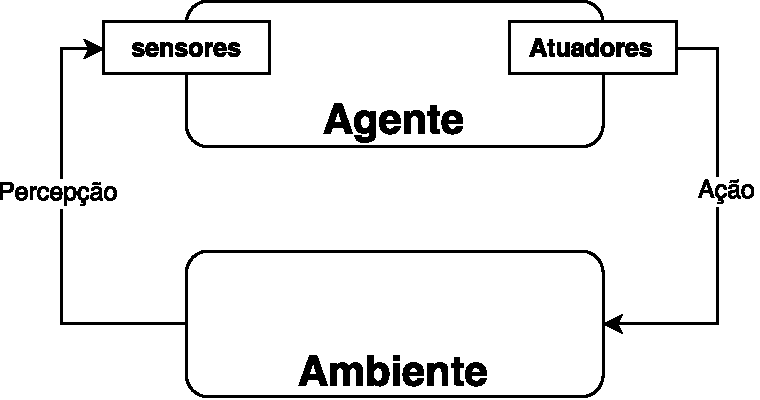
\includegraphics[width=0.5\textwidth]{fig/agente.pdf}
	\caption{Representação de um agente}
	\label{fig:agente}
\end{figure} 

O agente deve agir de forma autônoma, para isso ele deve ser capaz de aprender a lidar com situações proporcionadas pelo ambiente, com o intuito de realizar ações em busca do seu objetivo. O agente precisa de três características para conseguir ser autônomo \cite{agent1999}. São elas:
 
\begin{itemize}
	\item reatividade, para que os agentes sejam capazes de perceber o ambiente e suas mudanças a fim de levar o ambiente em consideração para a tomada de decisão das ações;
	\item pró-atividade, para que os agentes consigam ter a iniciativa em tomar as suas ações; e
	\item habilidade social, para que os agentes sejam capazes de interagir com outros agentes(humanos ou não).
\end{itemize}

As duas primeiras características são necessárias para que o agente consiga interagir com o ambiente. Um agente sendo reativo, ele consegue, a partir de uma mudança do ambiente, saber como ele deve se comportar. Sendo proativo, o agente pode antecipar suas ações em busca do seu objetivo.
Nem sempre um agente vai estar sozinho no ambiente, por esse motivo, a terceira característica é necessária para que o agente consiga interagir com outros agentes. Sistemas onde existem mais de um agente são chamados de sistema multi agentes. Nesses sistemas, os agentes interagem entre si, podendo ter objetivos em comum ou não. Sendo assim eles terão que cooperar ou negociar entre si \cite{intelligence2003modern}.

\section{Ambientes}

O agente deve se comunicar com um ambiente para conseguir alcançar seus objetivos. Mas um ambiente é composto por diversas propriedades que podem influenciar como o agente vai agir para chegar ao seu objetivo \cite{intelligence2003modern}. 

Nem sempre todas as informações do ambiente estarão disponíveis, por esse motivo o ambiente pode ser dito como completamente observável, parcialmente observável ou não observável, dependendo da informação disponibilizada. Um ambiente é dito completamente observável se, em qualquer instante de tempo, todas as informações relevantes do ambiente estão disponíveis para os sensores do agente. Caso haja alguma informação que não possa ser acessada, em algum instante de tempo, seja por causa da incapacidade do sensor do agente de captar essas informações ou pelo fato da informação simplesmente não ser disponibilizada, o ambiente é dito parcialmente observável. Agora, se o ambiente não disponibiliza nenhuma informação, o ambiente é tido como não observável \cite{ intelligence2003modern, agent1999}.   

O ambiente pode sofrer modificações, as modificações podem ser provenientes de ações realizadas pelos agentes, ou ainda por mudanças ocasionadas pelo próprio ambiente. O ambiente é determinístico se o estado gerado após a execução de uma ação, em todas as vezes que for executada, levar para o mesmo estado resultante, ou seja, o estado resultante é determinado pelo estado atual e a ação executada pelo agente. Se não há a certeza do estado resultante, o ambiente é estocástico. Quando o ambiente é não determinístico existem chances das ações dos agentes nem lembre levarem para os estados conhecidos \cite{intelligence2003modern}. 

Os estados do ambiente irão mudar ao longo do tempo, seja por uma ação feita por algum agente, ou por alguma mudança que possa ocorrer em razão de outro processo do ambiente. Se o ambiente sofre alguma alteração apenas quando o agente executa alguma ação, o ambiente é estático. Se o ambiente tem a capacidade de mudar independente de uma ação de um agente, o ambiente é dinâmico \cite{agent1999}.

Em sistemas multi agentes os agentes podem estar competindo ou cooperando entre si. O ambiente é competitivo quando os agentes estão competindo, como em um jogo de xadrez, por exemplo, ou o ambiente é cooperativo quando os agentes estão cooperando \cite{intelligence2003modern}.

\section{Arquiteturas de Agentes}


O tipo mais simples de agente é aquele que apenas reage a uma percepção vinda do ambiente. O agente escolhe suas ações baseado no que percebe no momento da decisão, sem levar em consideração ações já tomadas ou percepções anteriores. O agente apenas responde a uma percepção com uma ação, como se houvesse um clausula condicional que determinasse qual a ação a ser tomada se acontecer alguma coisa, como por exemplo, se estiver chovendo eu irei levar um guarda-chuva. A Figura~\ref{fig:agenteSimple} ilustra essa arquitetura. 

\begin{figure}[ht]
	\centering
	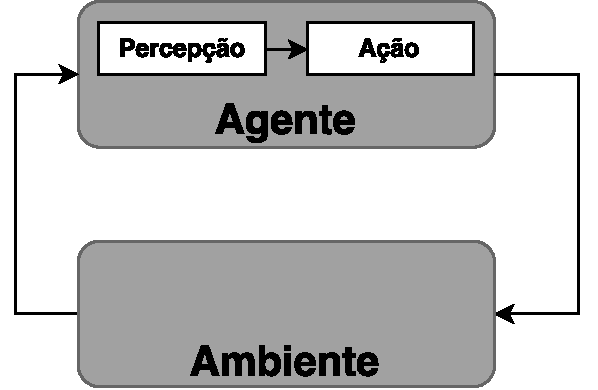
\includegraphics[width=0.4\textwidth]{fig/agentSimple.pdf}
	\caption{Arquitetura simples de um agente.}
	\label{fig:agenteSimple}
\end{figure} 


Este tipo de agente consegue ser simples, no entendimento e na sua utilização, mas a sua inteligência é limitada. Essa arquitetura é eficaz em ambientes completamente observáveis, pelo fato de que o agente precisa da percepção para realizar a sua ação \cite{intelligence2003modern}. A arquitetura pode ser usada, por exemplo, quando for preciso conhecer um conjunto de cidades, o agente após chegar a uma cidade, vai para a próxima cidade ao norte da cidade atual, quando não há norte ele vai para oeste. 

Na tentativa de aprimorar as decisões tomadas pelo agente, pode-se usar um estado interno para marcar qual a situação do ambiente. A informação representada no estado pode ser alguma informação que não consiga ser obtida por alguma percepção do ambiente ou de estados que já foram visitados pelo agente, por exemplo \cite{intelligence2003modern}. A Figura~\ref{fig:agenteModelbased} ilustra esta arquitetura. 

\begin{figure}[ht]
	\centering
	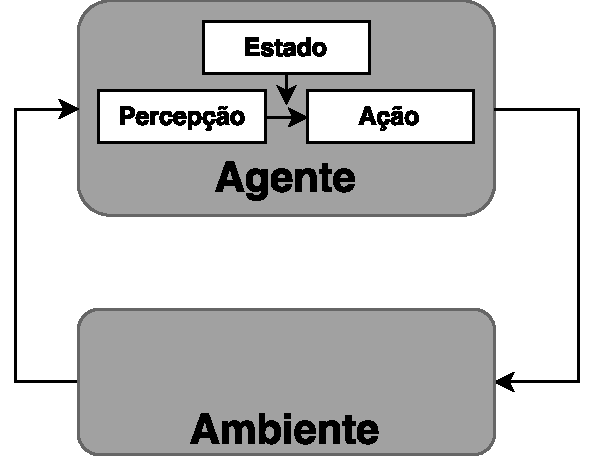
\includegraphics[width=0.4\textwidth]{fig/agentModel.pdf}
	\caption{Arquitetura de agentes com estados.}
	\label{fig:agenteModelbased}
\end{figure} 

Este tipo de arquitetura é eficaz para ambientes parcialmente observáveis, pelo fato de que o estado pode guardar informações relevantes para o agente \cite{intelligence2003modern}. No exemplo de conhecer as cidades, se guardar as visitas antigas, pode ajudar a não visitar novamente cidades que já tiverem sido visitadas. 

Dependendo do intuito do agente, conhecer o estado atual do ambiente não é suficiente. Além de estado, o agente pode precisar de uma informação para saber onde ele quer chegar, ou seja, um objetivo. Um objetivo é usado para descrever o que o agente está almejando alcançar. Para o agente conseguir alcançar o objetivo com uma melhor performance pode ser utilizado uma função de utilidade, nesta função é medido o "desejo" do agente em tomar determinada ação. Cada ação exercida pelo agente terá influência no valor de utilidade obtido \cite{intelligence2003modern}. Seguindo no exemplo, o objetivo pode ser visitar todas as cidades e a função de utilidade pode medir a distância entre as cidades, e assim podendo alcançar o objetivo com a menor distância percorrida. 



%!TEX root = volumeFinal.tex 
\chapter{\label{chap:busca}Busca}

Com o intuito de encontrar uma sequência de ações que um agente consiga alcançar o seu objetivo, é possível utilizar técnicas de busca.
O princípio da busca é encontrar uma solução de um problema através de um conjunto de ações que alcancem o objetivo desejado. 
Para utilizar as técnicas de busca é preciso formalizar o problema a ser resolvido e o objetivo a ser alcançado. Para utilizar as técnicas de busca, como entrada é recebido um problema e como resolução é retornado um conjunto de ações. 
Um problema pode ser definido por cinco componentes \cite{intelligence2003modern}: 

\begin{itemize}
	\item $s_{0}$, o estado inicial, onde o agente inicia no ambiente;
	\item ações, conjunto das possíveis ações disponíveis no agente;
	\item $resultado(s, a)$, um modelo de transição, que define o estado resultante após a execução da ação a no estado s;
	\item $objetivo(s)$, verifica se o estado é o objetivo do agente; e
	\item custo do caminho, uma função que define um valor numérico para cada ação realizada em um estado. Essa função pode ser denotada por $c(s, a, s')$, onde s é o estado atual do agente, a é a ação que será aplicada ao estado s e $s'$ é o estado resultante aplicando o modelo de transição resultado(s, a). 
\end{itemize}   


Esses elementos são necessários como entrada para que as técnicas de busca consigam ser utilizadas. As técnicas de busca visam encontrar a solução para esse problema, ou seja, a sequência de ações que leve ao objetivo. 
A solução é obtida quando o agente iniciando no estado inicial do ambiente $s_{0}$, utiliza o modelo de transição $resultado(s, a)$, através das ações aplicadas nos estados, para chegar a um estado onde satisfaça o objetivo do agente $objetivo(s)$.
Existem diferentes técnicas para encontrar uma solução. As diferentes técnicas podem encontrar caminhos diferentes para o mesmo problema, isso vem do fato de que o custo do caminho, quando levado em consideração, pode encontrar uma solução ótima, o que significa que a sequência de ações encontrada é a que tem o menor custo de caminho entre todas as soluções \cite{intelligence2003modern}.

Com a finalidade de exemplificar um problema de busca, considere o mapa apresentado na figura \ref{fig:mapabusca}. Cada círculo representa uma cidade, e as linhas entre as cidades são estradas que ligam as cidades uma a outra. A única ação possível é a de se locomover entre as cidades que tenham ligação. O estado inicial é a cidade de São Jerônimo. O resultado do modelo de transição, é a cidade resultante após se locomover. O objetivo do agente é chegar na cidade de Porto Alegre e o custo de cada ação é o valor definido em cima de cada transição. 

\begin{figure}[ht]
	\centering
	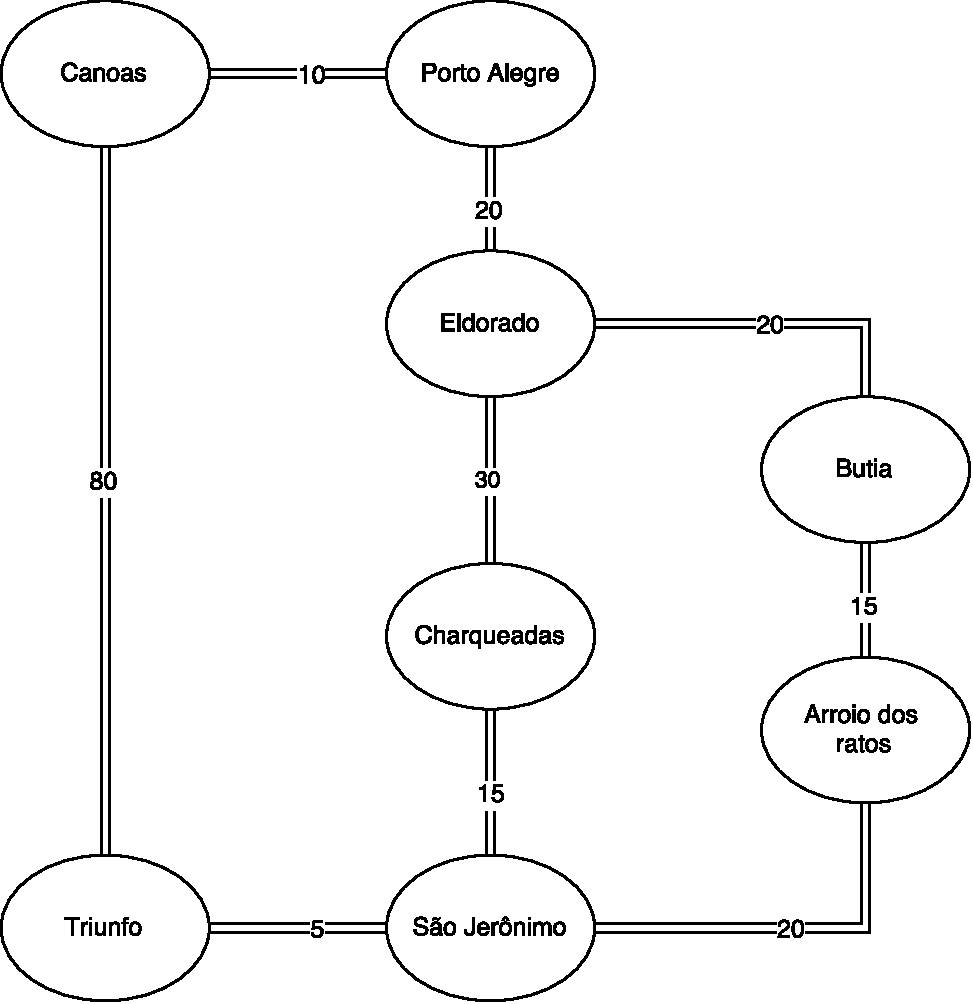
\includegraphics[width=0.6\textwidth]{fig/mapabusca.pdf}
	\caption{Mapa para o exemplo de problema de busca}
	\label{fig:mapabusca}
\end{figure} 

Para atingir o objetivo é preciso tentar os possíveis caminhos até o objetivo. Digamos que o agente comece sua viagem indo para a cidade de Triunfo, para nós(humanos) é intuitivo que a escolha não foi a melhor escolha para iniciar, mas a técnica só terá como saber após realizar todas as possíveis opções de caminhos, ou se utilizar uma técnica que utilize uma função de heurística, levando em consideração os custos dos caminhos, que acrescentam um conhecimento extra para a resolução do problema \cite{intelligence2003modern}.

\section{Busca adversaria}

Jogos são difíceis de resolver com técnicas de IA, pois eles requerem a habilidade de tomar algum tipo de decisão, e as técnicas comuns as vezes não são satisfatórias, seja pelo fato do conjunto de estados possíveis de se atingir ser muito grande, ou pelo curto espaço de tempo para tomar essa decisão.
A busca adversaria é utilizada nos jogos que estão situados em ambientes competitivos e de multi agentes. Em um jogo o jogador, preferencialmente, não informa suas jogadas previamente, assim tornando o ambiente imprevisível. Os objetivos dos jogadores entram em conflito, pois ambos estão em busca da vitória. 
Com o intuito de resolver esse problema é possível gerar uma solução de contingência para tentar antecipar as jogadas do adversário \cite{intelligence2003modern}. 

As técnicas de busca adversária utilizam uma variação da definição de um problema de busca comum. Os componentes devem se adequar ao ambiente competitivo. Por esse motivo os componentes são redefinidos como:

\begin{itemize}
	\item $s_{0}$, sendo o estado inicial, que especifica como o jogo se configura no início;
	\item $players(s)$, define qual jogador tem o movimento no estado $s$;
	\item $actions(s)$, conjunto das ações possíveis em um estado $s$;
	\item $result(s, a)$, um modelo de transição, que define o resultado da ação $a$ a aplicada ao estado $s$;
	\item $terminal(s)$, verifica se o estado $s$ é um estado onde o jogo termina; e
	\item $utility(s,p)$, define um valor numérico, representando o lucro do jogador $p$ ao atingir o estado terminal $s$.
\end{itemize}

Com esses componentes descritos é possível formalizar o que é uma árvore de jogadas. A árvore de jogados ou \textit{game tree} contém os estados do jogo e os movimentos possíveis em cada estado. A \textit{game tree} é composta pelo estado inicial $s_{0}$, as ações $action(s)$ e o modelo de transição $result(s, a)$, e possui uma profundidade $d$, que indica o nível máximo da árvore. 
A árvore representa em cada nodo um estado do jogo e em cada ligação os estados resultantes após a execução de cada ação possível para o estado. Considerando o jogo de jogo da velha, onde cada jogador realiza uma jogada de cada vez, uma \textit{game tree} que mostra parte das jogadas do jogo da velha é ilustrada na Figura~\ref{fig:jogodavelha}. O estado inicial do jogo é o campo vazio, a cada nível da árvore todas as possibilidades de jogadas são testadas, a profundidade $d$ dessa árvore chega a 9 quando ela estiver completa, pois a cada nível da árvore uma jogada é marcada no campo. 

\begin{figure}[ht]
	\centering
	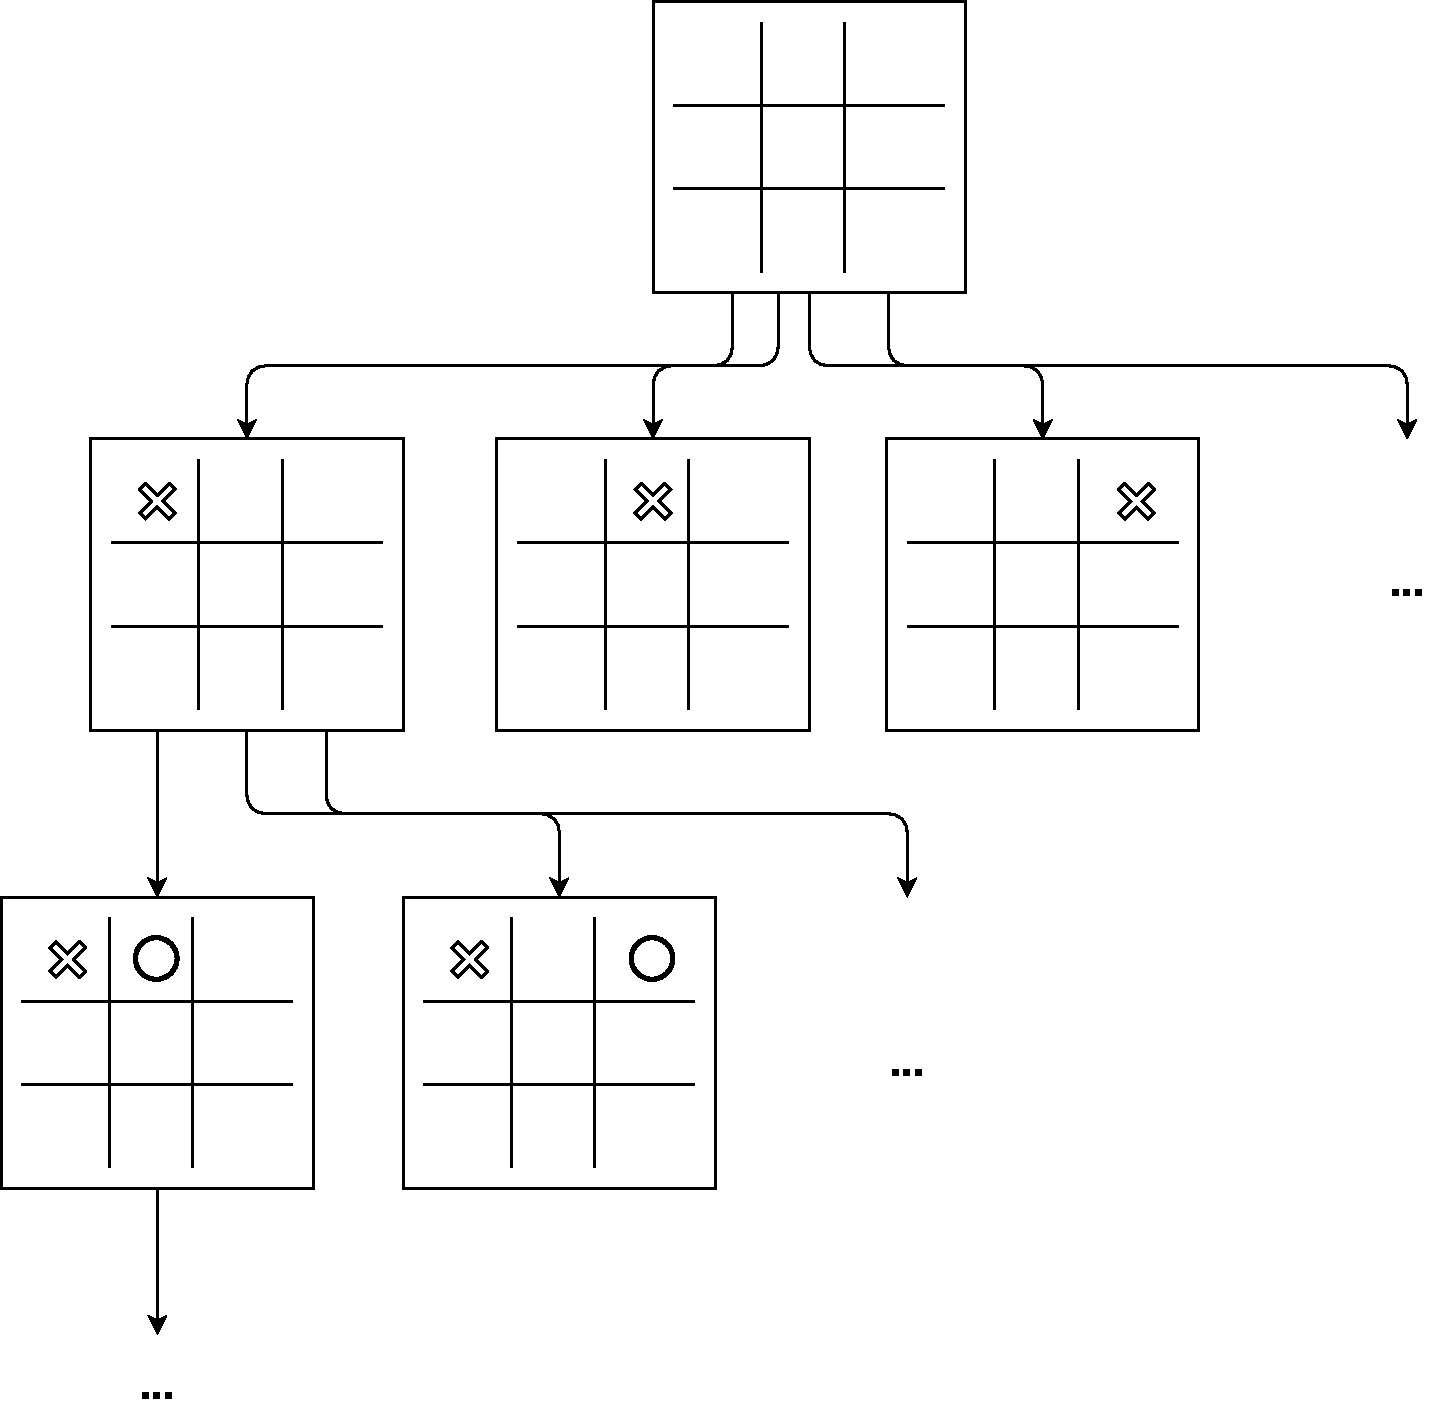
\includegraphics[width=0.5\textwidth]{fig/jogodavelha.pdf}
	\caption{Exemplo de um pedaço de uma \textit{game tree} sobre o jogo da velha}
	\label{fig:jogodavelha}
\end{figure} 

\section{Minimax search}

O algoritmo de \textit{minimax search} é utilizado como uma técnica de busca adversária. O objetivo do algoritmo é retornar a melhor jogada para o estado atual. Esse método considera dois agentes, chamados de \textsc{Max} e \textsc{Min}, onde o jogador \textsc{Max} representa a perspectiva do agente que está tentando maximalizar suas ações em relação ao agente \textsc{Min}, que representa o agente adversário do jogador \textsc{Max}. O algoritmo alterna entre jogadas de \textsc{Max} e \textsc{Min} \cite{intelligence2003modern}. 

O algoritmo utiliza a \textit{game tree} para analisar todos os estados possíveis do jogo, e assim decidir qual a ação que quando aplicada ao seu estado atual, trará um melhor benefício no futuro, se caracterizando a melhor jogada. Os nodos folhas da árvore, que representam o final do jogo, contém um valor de utilidade. Os valores mais altos são as melhores jogadas para \textsc{Max}, e consequentemente, os valores menores são melhores para \textsc{Min}. Ao chegar no final da árvore o algoritmo consegue o valor de utilidade para aquele cenário do jogo, quando isso acontece, o algoritmo faz o caminho inverso na árvore analisando os outros possíveis cenários \cite{intelligence2003modern}. A Figura~\ref{fig:gametree} ilustra esse processo.

\begin{figure}[ht]
	\centering
	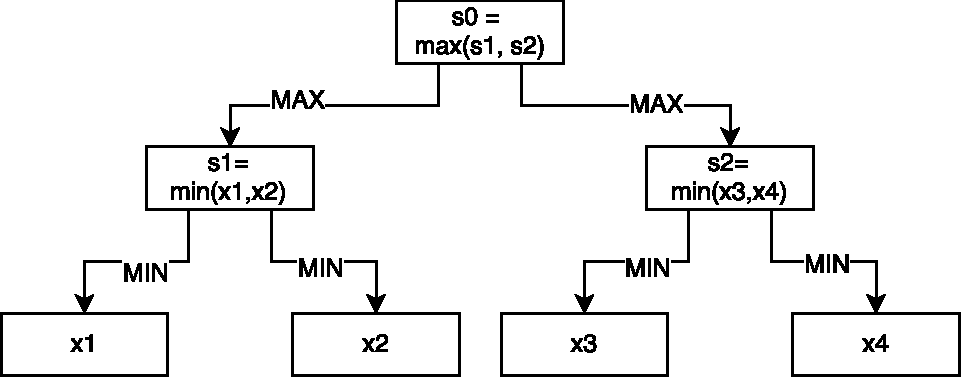
\includegraphics[width=0.6\textwidth]{fig/gametree.pdf}
	\caption{Exemplo de game tree utilizando \textit{minimax search}}
	\label{fig:gametree}
\end{figure} 

O método de \textit{minimax search} assume que os todos os jogadores como sendo racionais, com isso o algoritmo considera que as ações tomadas pelos agentes sempre realizarão uma jogada para tentar ganhar o jogo. O algoritmo de \textit{minimax search} é ilustrado no Algoritmo~\ref{alg:minimax}. O algoritmo tem como retorno a melhor ação a ser realizada no estado atual. As funções presentes nas linhas~\ref{alg:minimax:max} e ~\ref{alg:minimax:min} são utilizadas para calcular a jogada na visão de \textsc{Max} e \textsc{Min} respectivamente.
A função presente na linha~\ref{alg:minimax:minimax} é utilizada para iniciar a recursão e ao final retornar o melhor valor de utilidade para o jogador \textsc{Max}.

\begin{algorithm}
	\caption{Minimax Search}
	\label{alg:minimax}
	\begin{algorithmic}[1]	
		\Function{Minimax}{$state$} \label{alg:minimax:minimax}
		\State \Return $arg max_{action~ \in~ actions(s)}~ min\_value(result(state,  action)) $
		\EndFunction \\
		\Function {Max\_Value}{$state$}\label{alg:minimax:max}
		\If {$terminal(state)$}
		\State	\Return $utility(state)$
		\EndIf
		\State $v = -\infty$
		\ForAll{$action \in actions(state)$}
		\State $v = max(v, min\_value(result(state,action)))$
		\EndFor	
		\EndFunction \\
		\Function {Min\_Value}{$state$}\label{alg:minimax:min}
		\If {$terminal(state)$}
		\State	\Return $utility(state)$
		\EndIf
		\State $v = \infty$
		\ForAll{$action \in actions(state)$}
		\State $v = min(v, max\_value(result(state,action)))$
		\EndFor	
		\EndFunction
	\end{algorithmic}
\end{algorithm}


O algoritmo de \textit{minimax} deve explorar todo o espaço de estados para conseguir encontrar a ação que deve ser executada. A quantidade de estados possíveis, dependendo da situação, pode ser muito alta, no xadrez esse número chega a $10^{50}$, em um jogo de \textit{poker} no estilo \textit{texas holdem} esse número pode chegar a $10^{80}$. Geralmente, as ações devem ser tomadas em uma quantidade de tempo muito pequena. Por esse motivo, utilizar técnicas de busca para jogos pode ser um problema. Existem algumas abordagens que utilizam busca adversaria com um nível de abstração mais alto para tentar minimax esse problema \cite{ontanon2013survey}. 
%!TEX root = volumeFinal.tex 
\chapter{Planejamento}
\label{chap:planejamento}

A atividade de planejar alguma coisa é feita muitas vezes por dia. Algumas vezes esse planejamento é muito simples, como organizar as tarefas que serão feitas no próximo dia, outras vezes pode ser mais complexa como organizar uma viagem de final de ano. Planejar implica em elaborar uma sequência de ações com o intuito de alcançar um objetivo, ou seja, o processo de planejar consiste em organizar as ações, antecipando os resultados esperados de cada ação, com o intuito de conquistar um objetivo. 

O planejamento, na área da IA, é uma sub área de estudo, onde ele é usado para encontrar um plano que resolva um problema especifico. Como os ambientes nem sempre possuem as mesmas características, existem diferentes técnicas que são usadas para construir um plano.

\section{Planejamento automatizado}
\label{sec:classicalPlanning}

Planejamento automatizado estuda o processo de geração de planos computacionalmente. O objetivo do planejamento é encontrar uma sequência de ações que solucione um problema, a sequência de ações encontrada é chamada de plano. Para construir um plano é utilizado um planejador. O planejador recebe uma descrição formal de um problema de planejamento, e tenta solucionar esse problema, para isso pode ser utilizado algoritmos de buscas e heurísticas~\cite{ghallab2004automated}\cite[Capítulo 10]{intelligence2003modern}.

\subsection{Representação de um problema de planejamento}
\label{subsec:classicalPlanningRep}

Uma das maneiras de representar um problema de planejamento é utilizando lógica proposicional.
A lógica proposicional é expressada através de sentenças atômicas, que são compostas de proposições. 
Cada proposição pode assumir um valor de verdadeiro ou falso. 
Por exemplo, queremos representar que a lâmpada está apagada, para isso pode ser utilizado a proposição $apagada$, se a lâmpada estiver apagada, a proposição assume o valor de verdadeiro. Junto com as proposições podem ser usados conectivos lógicos, como negação (\textit{not}) $\neg$, conjunção (\textit{and}) $\wedge$ e disjunção (\textit{or}) $\vee$. 
No exemplo da luz, se queremos saber se a luz está apagada e a TV está ligada, podemos representar por $apagada~ \wedge~ ligada$. 
A lógica proposicional pode ser considerada simples, mas ela serve de base para as lógicas mais expressivas~\cite[Capítulo 10]{intelligence2003modern}. 

Como a lógica proposicional tem expressividade limitada, é preciso utilizar uma lógica que consiga expressar mais sobre os estados do ambiente que desejamos representar. 
A lógica de primeira ordem (LPO) estende a lógica proposicional, e diferente da lógica proposicional a LPO consegue representar relação entre preposições, ou seja, as preposições podem ter aridade mais que um, um exemplo pode ser um objeto estar sobre o outro ($sobre(A,B)$). Uma outra diferenças da LPO é a possibilidade de utilizar quantificadores para demonstrar fatos comuns sobre as preposições, como objetos que tenham a mesma cor ($\forall x~ azul(x)$).

A descrição formal de sentenças em LPO é composta por um predicado seguido de uma lista de termos, denotada por $p(t_{0}, t_{1}, ..., t_{n})$. 
Um predicado se refere a uma relação existente entre os termos. 
Os termos são objetos que se referem a objetos definidos, indefinidos ou a funções \cite[Capítulo 10]{intelligence2003modern}. 
No exemplo da lâmpada, podemos dizer que a lâmpada da cozinha está apagada, representado por $apagada(cozinha)$. 
Ou ainda podemos dizer que a lâmpada do quarto está apagada e a TV da sala está ligada, $apagada(quarto)~ \wedge~ ligada(sala)$.  

\subsection{Formalização de um problema de planejamento}
\label{subsec:classicalPlanningForm}

Alguns conceitos são importantes para entender a formalização de um problema de planejamento. 
Os estados são um conjunto de átomos que não podem ser divididos em sub-fórmulas, esses átomos assumem valores de verdadeiro ou falso, dependendo da interpretação do ambiente.
As ações alteram o estado do ambiente. Para que elas sejam aplicadas é preciso que um conjunto de precondições seja satisfeito, se for é aplicado um conjunto de efeitos sobre o ambiente~\cite[Capítulo 10]{intelligence2003modern}.
Um exemplo é mover um objeto de um lugar para o outro, precisamos de um predicado que defina que um objeto está em determinado lugar. Esse exemplo é representado abaixo:

\begin{itemize}
	\item Ação: $move(from, to)$
	\item Precondição: $at(from)$
	\item Efeito: $\neg at(from) \wedge at(to)$
\end{itemize}

Uma ação $a$ é aplicável em um estado $s$, se todas as precondições forem satisfeitas no estado $s$. 
O resultado gerado pela execução de $a$ no estado $s$ é um novo estado $s'$, nesse estado é aplicado todos os efeitos, removendo os predicados negativos e adicionando os positivos~\cite{meneguzzi2015planning}.

Os operadores são definido como $op = (nome(t), precondições(p), efeitos(p)$. 
O $nome(t)$ é o nome do operador e $t$ é o conjunto de termos que compõem as precondições e os efeitos. $precondições(p)$ é o conjunto de predicados que representam as precondições do operador. $efeitos(p)$ é o conjunto de predicados que serão o resultado após a execução do operador;
Todas os operadores disponíveis para a resolução do problema formam a descrição das ações~\cite{ghallab2004automated}.
 
Como nas técnicas de busca, em planejamento também é necessário ter uma descrição do problema.
Formalmente, um problema de planejamento pode ser descrito como $P = (\Sigma, s_{0}, g)$, onde $\Sigma$ é a descrição do problema com as ações disponíveis, $s_{0}$ é o estado inicial onde o problema começa e $g$ é o objetivo~\cite{ghallab2004automated}. 
Voltando ao exemplo do Capítulo~\ref{chap:busca}, onde um agente tenta chegar a cidade de Porto Alegre partindo da cidade de São Jerônimo, podemos formalizá-lo como:

\begin{itemize}
	\item \textbf{estado inicial} ($s_{0}$) = $At(S$\~a$o~Jer$\^o$nimo)$;
	\item \textbf{objetivo} ($g$) = $At(Porto~Alegre)$; e
	\item \textbf{domínio} ($\Sigma$) = 
	\begin{itemize}
		\item nome: $move(cityA, cityB)$
		\item precondições: $at(cityA) \wedge link(cityA, cityB)$
		\item efeitos: $\neg at(cityA)~ \wedge at(cityB)$.
	\end{itemize}
\end{itemize}


O processo de geração do plano é feito pelo planejador. 
Um plano é uma sequência de operadores gerada a partir de um problema que, quando executada partindo do estado inicial, modifica o estado de forma que o objetivo seja válido no estado resultante. 
A Figura~\ref{fig:planmodelo} ilustra o comportamento do planejador.
Para realizar a formalização de um problema de planejamento é preciso definir alguns conceitos.

\begin{figure}[ht]
	\centering
	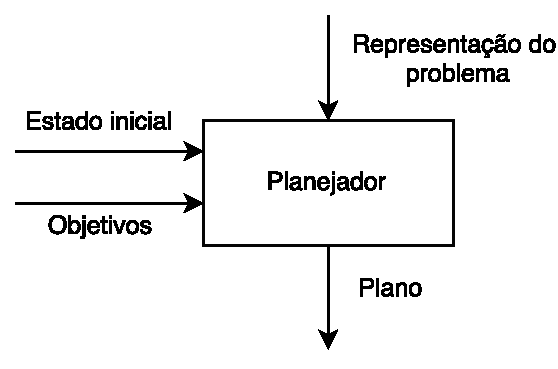
\includegraphics[width=0.4\textwidth]{fig/modelo.pdf}
	\caption{Problema de planejamento clássico.}
	\label{fig:planmodelo}
\end{figure} 

Um plano é considerado ótimo quando não há nenhum outro plano que atinga o objetivo utilizando um número menor de ações.
Uma forma de gerar planos ótimos é utilizando técnicas de busca combinado com alguma heurística que seja independente de domínio.
Uma heurística deve ser computacionalmente eficiente e ter precisão para que a geração do plano seja eficiente~\cite{helmert2007flexible}.

\section{Planejamento hierárquico} 
\label{sec:htnPlanning}

O planejamento clássico consegue gerar planos ótimos.
Mas o tratamento de problemas de grande complexidade ou com o espaço de estados grande pode se tornar intratável.
Isso acontece por conta do poder computacional necessário para que o plano consiga ser gerado.
O planejamento clássico possui uma expressividade limitada, pois não é possível representar quando uma ação irá ocorrer, por exemplo~\cite[Capítulo 11]{intelligence2003modern}.
Como alternativa para esses problemas foi proposto o planejamento hierárquico, chamado de \textit{Hierarchical Task Network} (HTN). 
O planejamento HTN se diferencia do planejamento clássico na forma como os planos são gerados~\cite{ghallab2004automated}. 
Enquanto no planejamento clássico é necessário ter heurísticas para a geração de planos, em planejamento HTN é possível expressar conhecimento de domínio junto com os operadores, isso faz com que as ações sejam tratadas em mais alto nível.  
O conhecimento de domínio contém informações que determinam o espaço de estados possível para determinado ambiente. O planejador utiliza o conhecimento de domínio para percorrer entre os estados e encontrar os planos possíveis. Para isso o conhecimento de domínio deve conter informações relativas as ações, disponíveis no ambiente, e as possíveis transições de estados~\cite[Capítulo 11]{intelligence2003modern}.

O objetivo do planejamento HTN é produzir uma sequência de ações que executam determinada tarefa $t$. 
As tarefas são completadas decompondo tarefas não primitivas em tarefas menores até só restarem tarefas primitivas.  
As tarefas primitivas são análogas as ações executáveis em planejamento clássico, e expressam uma atividade que o agente possa executar diretamente no ambiente~\cite[Capítulo 11]{intelligence2003modern}. 
Já as tarefa não primitiva representam objetivos que o agente deve alcançar com o intuito de decompor as tarefas não primitivas em primitivas. 
O exemplo da seção anterior de mover um objeto de lugar é um exemplo de tarefa primitiva, pois altera o estado do ambiente, podendo ser representado em HTN como: \texttt{(move~ ?from~ ?to)}. 
Um exemplo de tarefa não primitiva é realizar uma viagem de carro, para conseguir completar essa tarefa é necessário fazer a revisão do carro, arrumar as malas e colocar tudo dentro do carro, que pode ser representado por \texttt{(travelByCar ~?car~ ?stuffs)}. 

Para iniciar a geração de um plano HTN, deve ser usado como início uma tarefa de ligação. 
Uma tarefa de ligação HTN é definida como $w = (T, C)$, onde $T$ é um conjunto de tarefas a ser completadas e $C$ é um conjunto ordenado de restrições sobre as tarefas $T$. 
As restrições estabelecem a ordem com que as tarefas $T$ devem ser executadas. 

Um domínio de planejamento HTN é um par $D = (A, M)$, onde $A$ é um conjunto de predicados, que representam estados no ambiente, e $M$ um conjunto finto de métodos \cite{meneguzzi2015planning}. 
Um método é utilizado para decompor tarefas não-primitivas em primitivas. 
Um método é representado por $m = (p, t, w)$, onde $p$ é uma precondição que estabelece o que deve estar presente no estado atual para que a tarefa $t$ consiga ser decomposta por uma tarefa de ligação $w$ \cite{ghallab2004automated}. 
Considerando o exemplo anterior de viajar de carro, a Figura~\ref{fig:htnmethod} ilustra esse método, sendo a tarefa em cinza uma tarefa não primitiva, que posteriormente também será decomposta. 
O conjunto de tarefas que faz parte da tarefa de ligação está representada pelas sub tarefas, e a ordem caracteriza as restrições. 

\begin{figure}[ht]
	\centering
	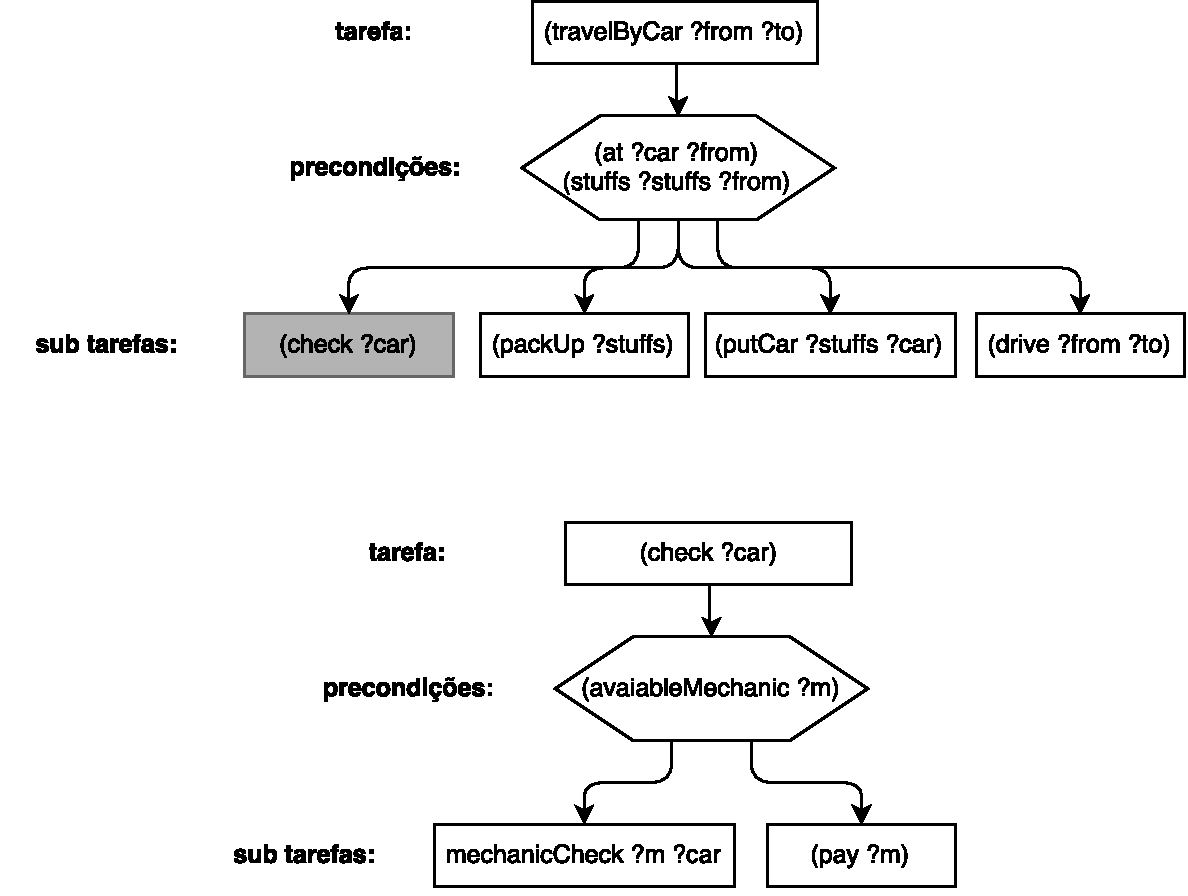
\includegraphics[width=0.7\textwidth]{fig/htnmethod.pdf}
	\caption{Exemplo de método HTN.}
	\label{fig:htnmethod}
\end{figure} 

Um problema de planejamento HTN $P$ é definido como $P = (d, I, D)$, onde $D$ é um domínio, $d$ é a tarefa de ligação inicial e $I$ é um estado inicial como no planejamento clássico. 
O processo de geração de um plano utilizando planejamento HTN consistem em encontrar um método que consiga ser aplicado na primeira tarefa de $d$, isso faz com que seja gerado uma tarefa de ligação diferente $d'$, onde a primeira tarefa foi decomposta. 
Esse processo continua, agora aplicado a $d'$, até que todas as tarefas sejam primitivas \cite{meneguzzi2015planning}. 
Se em algum ponto, nenhum método consiga ser aplicado, o planejador deve realizar um retrocesso(\textit{backtracking}), que consiste em voltar a um $d$ anterior a ponto de conseguir aplicar outra decomposição \cite[Capítulo 11]{intelligence2003modern}. 
É possível representar a busca do plano por uma árvore $N$, na qual os nodos são tarefas ou métodos. 
Cada tarefa não-primitiva pode ter apenas um filho, que deve ser um método. 
Cada método deve ter um filho para cada uma das suas sub tarefas. 
Tarefas primitivas não podem ter filhos, o que significa que elas não podem ser decompostas. 
Uma árvore totalmente decomposta, é onde todas as folhas de $N$ são tarefas primitivas \cite{ontanon2015adversarial}. 
A Figura~\ref{fig:htnmethodtree} ilustra a árvore de resolução do exemplo anterior.

\begin{figure}[ht]
	\centering
	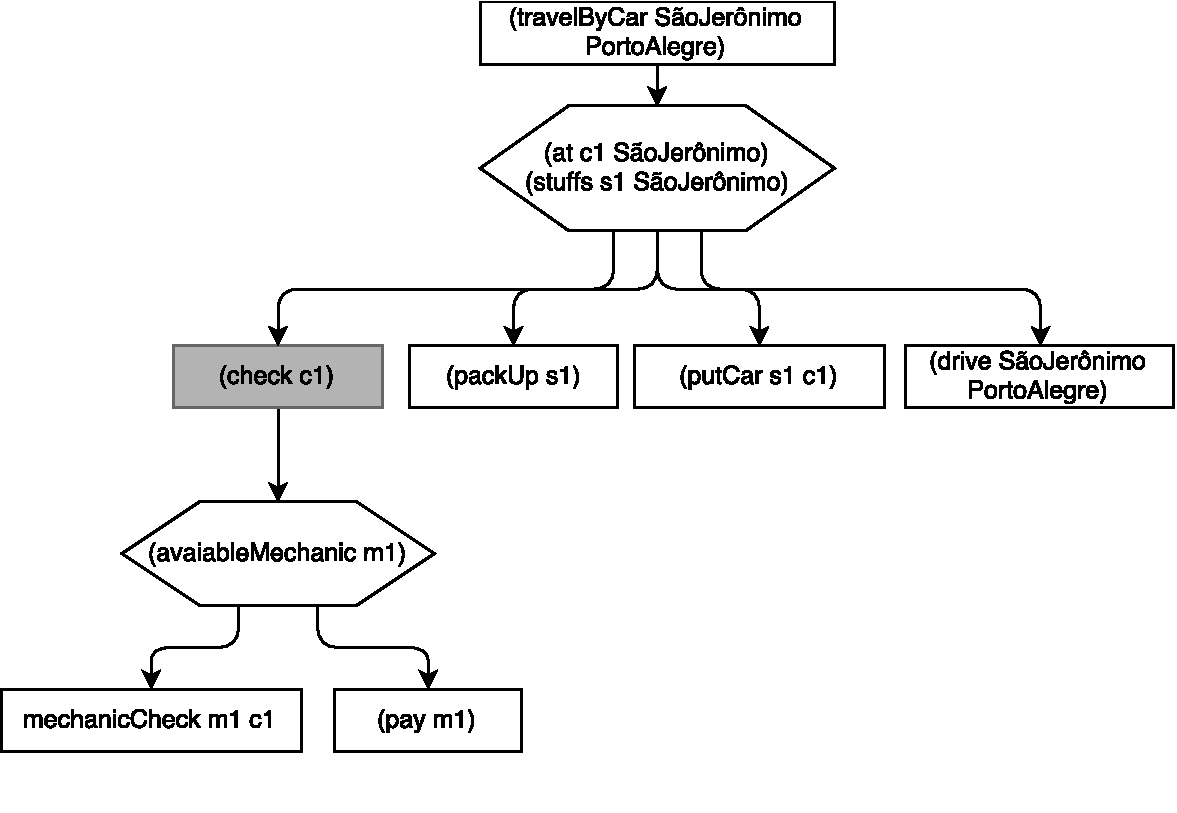
\includegraphics[width=0.7\textwidth]{fig/htnmethodresult.pdf}
	\caption{Arvore de resolução HTN.}
	\label{fig:htnmethodtree}
\end{figure}

O algoritmo de \textit{Total-order Forward Decomposition} (TFD) é utilizado para gerar um plano a partir de uma rede de tarefas inicial com ordenação total, como detalhado no Algoritmo~\ref{alg:tfd}.
O algoritmo gera as ações na mesma ordem que serão executadas, então a cada vez que uma tarefa é alcançada, tudo que antecede a mesma já foi planejado \cite{ghallab2004automated}.
 
\begin{algorithm}
	\caption{Total-order Forward Decomposition}
	\label{alg:tfd}
	\begin{algorithmic}[1]		
		\Function {TFD}{$s, <t_{1}, ...,t_{k}>, O, M$}
			\If {$k = 0$}
				\State	\Return $<>$
			\EndIf
			\If {$t_{1}$ é primitivo}
				\State $ativo = \{(a, b)~ |$ $a$ é uma instancia de $O$ e é aplicável a $s$ e b é uma substituição que torna $a$ relevante para $b(t_{1})\}$
				\If {$ativo = \emptyset$}
					\State \Return falha
				\EndIf
				\State escolhe algum par $(a, b) \in active$
				\State $\pi = TFD(\gamma(s, a), b(<t_{2}, ..., t_{k}>, O, M)$
				\If {$\pi = falha$}
					\State \Return falha
				\Else 
					\State \Return $a . \pi$
			\EndIf
			
			\ElsIf {$t_{1}$ é não primitiva}
				\State $ativo = \{m |~ m$ é aplicável a $s$ e $m \in M\}$
				\If {$ativo = \emptyset$}
					\State \Return falha
				\EndIf
				\State escolhe algum par $(m, b) \in active$
				\State $w =~ $subtarefas$(m).b(<t_{2}, ..., t_{k}>)$
				\State \Return $TFD(s, w, O, M)$
				\EndIf
		\EndFunction
	\end{algorithmic}
\end{algorithm}

\section{Adversarial hierarchical-task network} \label{sec:ahtn}

\textit{Adversarial hierarchical-task network} (AHTN) é um algoritmo desenvolvido para lidar com o problema do grande fator de ramificação dos jogos em tempo real~\cite{ontanon2015adversarial} utilizando conhecimento de domínio no estilo de planejamento HTN. 
Nele são combinados técnicas de HTN com o algoritmo \textit{minimax search}. 
O algoritmo assume jogos totalmente observáveis, baseados em turno e determinísticos. 

O Algoritmo~\ref{alg:ahtn}~\cite{ontanon2015adversarial} é a representação da técnica de AHTN, e assume que existem dois jogadores, \textsc{Max} e \textsc{Min}, como no algoritmo de \textit{minimax search} apresentado na Seção~\ref{sec:minimax}. 
O algoritmo também assume uma busca em uma árvore com uma máxima profundidade $d$. 
O intuito do algoritmo de AHTN é gerar os melhores plano para \textsc{Max} e para \text{Min}, junto com o resultado de uma função de avaliação para quando os planos chegam a um estado terminal. 

\begin{algorithm}
	\caption{Adversarial hierarchical-task network}
	\label{alg:ahtn}
	\begin{algorithmic}[1]		
		\Function {AHTNMax}{$s, N_{+}, N_{-}, t_{+}, t_{-}, d$}
		\If {$terminal(s) \vee d \leq 0$}\label{alg:lin:firstLine}
		\State	\Return $(N_{+}, N_{-}, e(s))$
		\EndIf
		\If {$nextAction(N_{+}, t_{+}) \neq \perp$} \label{alg:ahtn:nexaction}
		\State $t = nextAction(N_{+}, t_{+})$ 
		\State \Return $\Call{AHTNMin}{(\gamma(s,t), N_{+}, N_{-}, t, t_{-}, d-1)}$ \label{alg:ahtn:troca}
		\EndIf
		\State $N_{+}^{*} = \perp, N_{-}^{*} = \perp, v^{*} = -\infty$
		\State $\aleph = decompositions_{+}(s, N_{+}, N_{-}, t_{+}, t_{-})$ \label{alg:decompositions}
		\ForAll{$N \in \aleph$} \label{alg:ahtn:for}
		\State $(N^{'}_{+}, N^{'}_{-}, v^{'}) = AHTNMax(s, N, N_{-}, t_{+}, t_{-}, d)$
		\If{$v^{'} > v^{*}$}
		\State $N_{+}^{*} = N^{'}_{+}, N_{-}^{*} = N^{'}_{-}, v^{*} = v^{'} $
		\EndIf
		\EndFor		
		\State \Return $(N_{+}^{*}, N_{-}^{*}, v^{*} )$
		\EndFunction
	\end{algorithmic}
\end{algorithm}

O algoritmo de AHTN gera uma árvore das jogadas. Cada nodo da árvore é definido por uma tupla $(s, N_{+}, N_{-}, t_{+}, t_{-})$, onde $s$ é o estado corrente do ambiente, $N_{+}$ e $N_{-}$ são a representação de planos HTN para os jogadores \textsc{Max} e \textsc{Min}, respectivamente, $t_{+}$ e $t_{-}$ representam ponteiros para qual parte do plano HTN está sendo executada, sendo $t_{+}$ para uma tarefa de $N_{+}$ e $t_{-}$ para uma tarefa de $N_{-}$. Cada nodo da árvore representa um estado do jogo~\cite{ontanon2015adversarial}.

O algoritmo alterna a perspectiva dos jogadores sempre que existir uma tarefa primitiva no plano atual, e assim avança na profundidade da árvore das jogadas. A função $AHTNMin$ é responsável pela mudança de perspectiva, e ela está presente no bloco que inicia na Linha~\ref{alg:ahtn:nexaction}. No mesmo bloco há a função \texttt{nextAction(N,t)}, que é responsável por verificar é possível a troca de perspectiva. Ela recebe como parâmetro um plano ($N$) e um ponteiro ($t$). Com isso ela retorna um ponteiro para a próxima tarefa primitiva, caso ainda não haja uma tarefa primitiva no plano, a função retorna $t = \bot$.

Caso não seja possível trocar de perspectiva, o algoritmo de AHTN decompõe o plano. O método $decompositions$ é responsável por decompor o plano atual a partir do estado do jogo na árvore. O método apenas adiciona novos planos que utilizem apenas um novo método ao plano atual. A chamada deste método ocorre na Linha~\ref{alg:decompositions} do algoritmo gerando novos planos.
O algoritmo utiliza as decomposições para comparar todos os planos gerados por uma função de avaliação. O plano que tiver a melhor função de avaliação é escolhido como melhor caminho. O plano escolhido é retornado junto com o resultado da função de avaliação. Este processo está presente na Linha~\ref{alg:ahtn:for}.

O plano pode acabar quando a profundidade limite for atingida, ou quando um estado terminal for alcançado.
Quando alguma dessas condições for alcançada, é retornado o plano das duas perspectivas e a função de avaliação para o estado do jogo atual. A Linha~\ref{alg:lin:firstLine} mostra essa condição.

A grande diferença entre o algoritmo de $AHTN$ e o algoritmo do \textit{minimax search}, é que as chamadas recursivas nem sempre se alternam entre \textsc{Max} e \textsc{Min}. 
O algoritmo troca de nodos \textsc{Max} para \textsc{Min} apenas quando os planos estão totalmente decompostos a ponto de gerar uma ação (Linha \ref{alg:ahtn:troca})~\cite{ontanon2015adversarial}.

A Figura~\ref{fig:ahtn}\footnote{Figura extraída de~\cite{ontanon2015adversarial}} é utilizada para exemplificar o funcionamento do algoritmo~\ref{alg:ahtn}. 
Na raiz da árvore há apenas uma tarefa não primitiva \textit{win} para ser decomposta, para os dois jogadores. 
Há duas decomposições que o jogador \textsc{Max} pode aplicar para seu plano HTN, resultando nos nodos $n_{1}$ e $n_{5}$. A decomposição $n_{1}$ não resulta em nenhuma ação primitiva, e por isso $n_{1}$ continua um nodo \textsc{Max}. Uma vez que o jogador \textsc{Max} decompõe seus planos e há tarefas primitivas para serem executadas (nodos $n_{2}$ e $n_{5}$), é o turno de \textsc{Min} decompor suas tarefas não primitivas. Após \textsc{Min} gerar suas ações, a profundidade máxima ($d = 2$) foi atingida (nodos $n_{3}$ e $n_{4}$). 
A função de avaliação $e$ é aplicada para cada um dos estados do jogo para determina o valor das folhas.

\begin{figure}[ht]
	\centering
	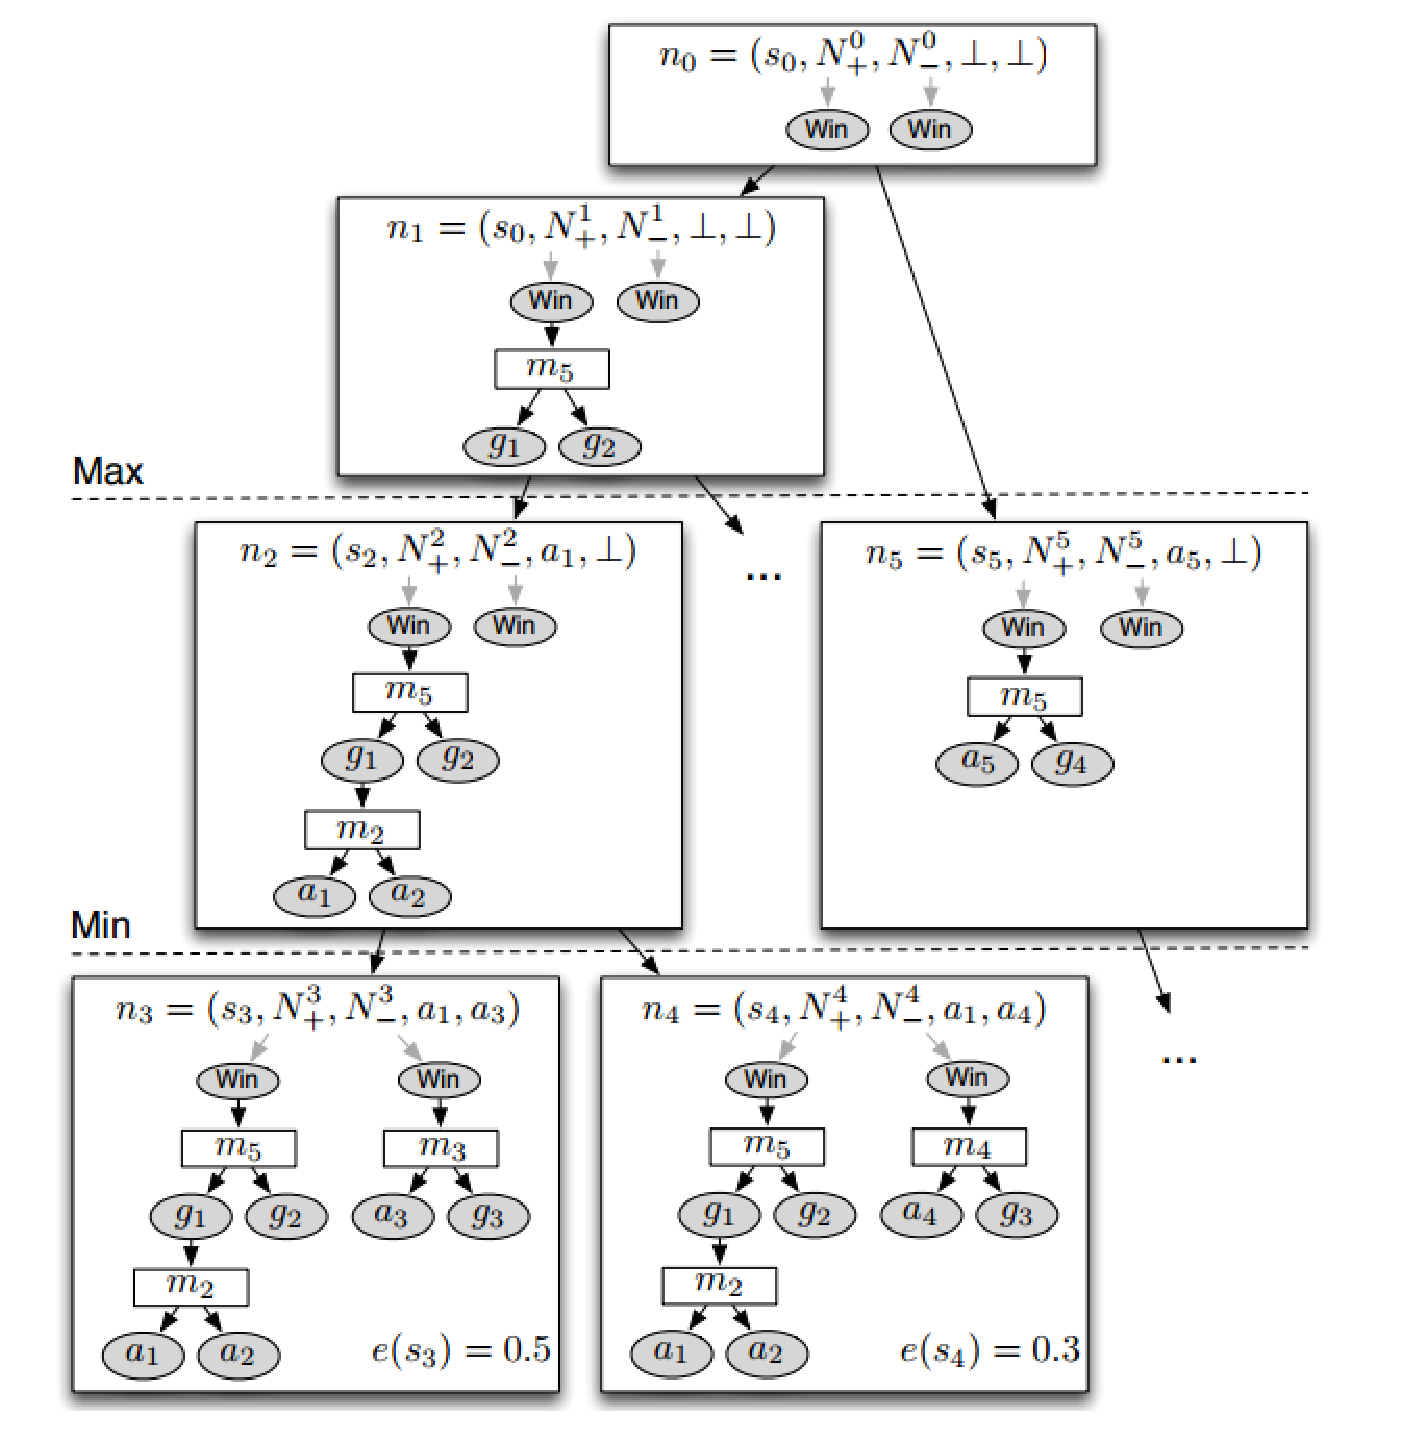
\includegraphics[width=0.8\textwidth]{fig/ahtn.pdf} 
	\caption{Árvore gerada pelo algoritmo de AHTN.}
	\label{fig:ahtn}
\end{figure}

O problema que o algoritmo de AHTN tenta lidar é o grande fator de ramificação e o pouco tempo para determinar a próxima ação do agente. O algoritmo utiliza planejamento através do conhecimento de domínio para diminuir a combinação de ações que não tem nenhuma chance de ser usadas em um jogo real~\cite{ontanon2015adversarial}. 

%!TEX root = volumeFinal.tex 

\chapter{\label{chap:proj}Projeto de Implementação}

Este capítulo apresenta o jogo MicroRTS, que foi escolhido para ser utilizado como plataforma para a implementação do algoritmo de AHTN. Este capítulo também apresenta como funciona o planejador HTN, que será utilizado para a geração de planos.

\section{MicroRTS}  \label{sec:microrts}

Jogos eletrônicos são muito populares, principalmente pela grande quantidade de gêneros, existem jogos de ação, aventura, esportes, estratégia, entre outros. Hoje em dia, os jogos buscam que quem jogue consiga ficar imerso no dentro do jogo, sem conseguir identificar um padrão nos jogadores fictícios, pois se não o jogo deixa de ser tão interessante. Para que isso aconteça, a IA é associada a diversos jogos, e é comum pensar que quanto mais complexa a IA aplicada dentro do jogo mais difícil jogo irá ficar, mas isso nem sempre é verdade. Não é sempre que uma IA complicada terá melhor desempenho do que uma mais simples. Uma boa IA, para jogos, é feita a partir do comportamento desejado para o jogo com os algoritmo certos~\cite{millington2009artificial}.

Jogos de estratégia em tempo real, também conhecidos por \textit{real-time strategy games} (RTS), é um subgênero de jogos de estratégia. 
Nesse gênero de jogo os jogadores devem construir uma base, buscar recursos, construir edificações, treinar unidades de ataques e aprimorar suas tecnologias.
O objetivo final do jogo é destruir uma ou mais bases inimigas. 
Alguns fatores que dificultam o desenvolvimento de IAs para jogos RTS. 
Os fatores estão relacionados com a complexidade dos jogos, pois os jogos RTS possuem um grande espaço de estados.
Além disso os jogadores realizam as jogadas ao mesmo tempo, fazendo com que cada jogador tenha um curto espaço de tempo para realizar as suas ações.
Por essa razão, não é possível traduzir automaticamente as técnicas de IA para jogos RTS sem algum tipo de abstração ou simplificação~\cite{ontanon2013survey, buro2012real}.

Um exemplo deste gênero é o MicroRTS\footnote{https://github.com/santiontanon/microrts}, uma simplificação de jogos como Starcraft\footnote{http://us.battle.net/sc2/pt/}. 
O MicroRTS foi desenvolvido por Santiago Ontañón~\cite{ontanon2013combinatorial} em Java para fins acadêmicos, com o intuito de aplicar e desenvolver técnicas de IA e para servir como prova de conceito para as técnicas criadas.
O MicroRTS consiste em dois jogadores tentando destruir a base adversaria. 
Para ganhar o jogo é preciso eliminar cada unidade e edificação do adversário. 
O jogo termina quando um dos dois jogadores não tem mais unidades, ou quando o jogo atinge o limite de tempo. 
A Figura~\ref{fig:microrts} mostra um exemplo de tela do jogo.

\begin{figure}[ht]
	\centering
	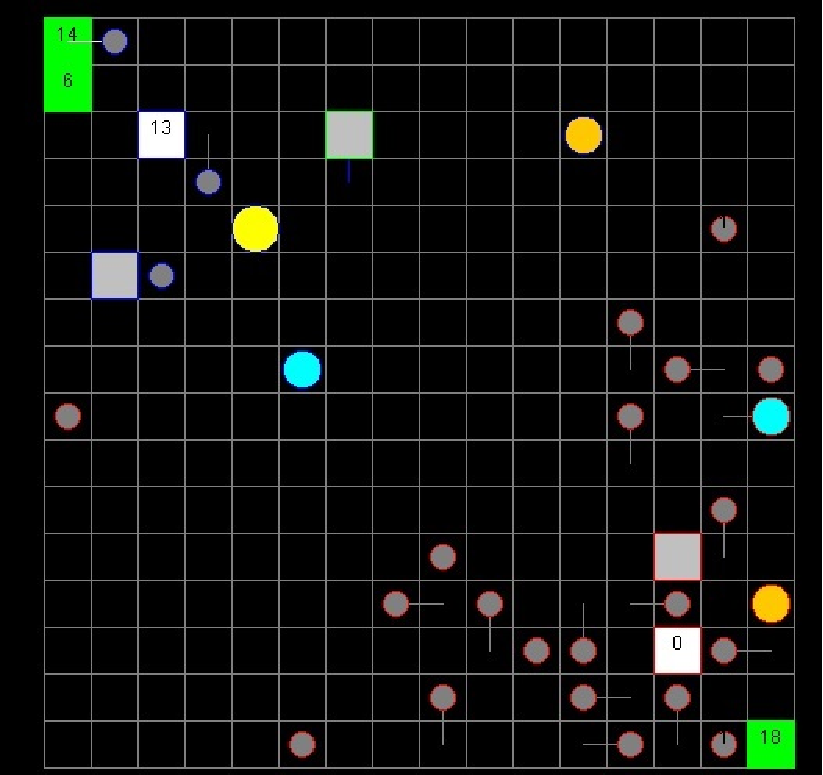
\includegraphics[width=0.5\textwidth]{fig/microrts.pdf}
	\caption{Um exemplo de tela do MicroRTS}
	\label{fig:microrts}
\end{figure} 

\subsection{Unidades e construções}
No MicroRTS existem quatro tipos de unidades no jogo, e cada uma foi descrita a seguir:

\begin{itemize}
	\item \textit{worker}, é responsável por coletar recursos e construir as edificações. Esta unidade também consegue lutar, mas possui um dano muito baixo;
	\item \textit{heavy}, unidade que pode apenas atacar. Ela possui um alto poder de ataque, mas sua velocidade é lenta;
	\item \textit{light}, unidade que pode apenas atacar. Ela possui um baixo poder de ataque, mas sua velocidade é rápida; e
	\item \textit{ranged}, unidade que pode apenas atacar. Ela possui um ataque de longa distância. 
\end{itemize} 

Para treinar as unidades é preciso ter recursos e edificações. 
No MicroRTS é preciso ter uma base que é a edificação principal. 
A base é responsável pela criação dos \textit{workers}.
Ela também é responsável pelo armazenamento dos recursos, que são necessários para treinar e construir tudo dentro do jogo. 
O quartel é responsável pela criação das unidades de ataque que podem apenas atacar. 
Ela pode ser construída apenas por \textit{workers} e é preciso utilizar uma quantidade de recurso para a sua construção. 
Os recursos são obtidos através dos \textit{workers}, que extraem recursos da base de recurso e armazenam na base. 

\subsection{Arquitetura}

O MicroRTS conta com cinco classes principais para funcionamento do jogo. 
Cada classe é responsável por um controle dentro do jogo.
As classes \textit{GameState} e \textit{PhysicalGameState} são responsáveis pelo controle das ações das unidades dentro do mapa.
A \textit{UnitTypeTable} é utilizada para associar cada unidade com as suas ações possíveis.
A classe \textit{PhysicalGameStatePanel} é responsável pela interface gráfica.
A classe \textit{GameVisualSimulation} é utilizada para unir todos os componentes do jogo, e configurar as informações de mapa, jogadores, humanos ou IAs, e tempo de duração da partida.
O diagrama de classes presente na Figura~\ref{fig:classes} ilustra como as classes se relacionam e seus principais métodos.

\begin{figure}[ht]
	\centering
	\frm[inline]{Nope, I want vector graphics, man! And text of a size that I can read.}
	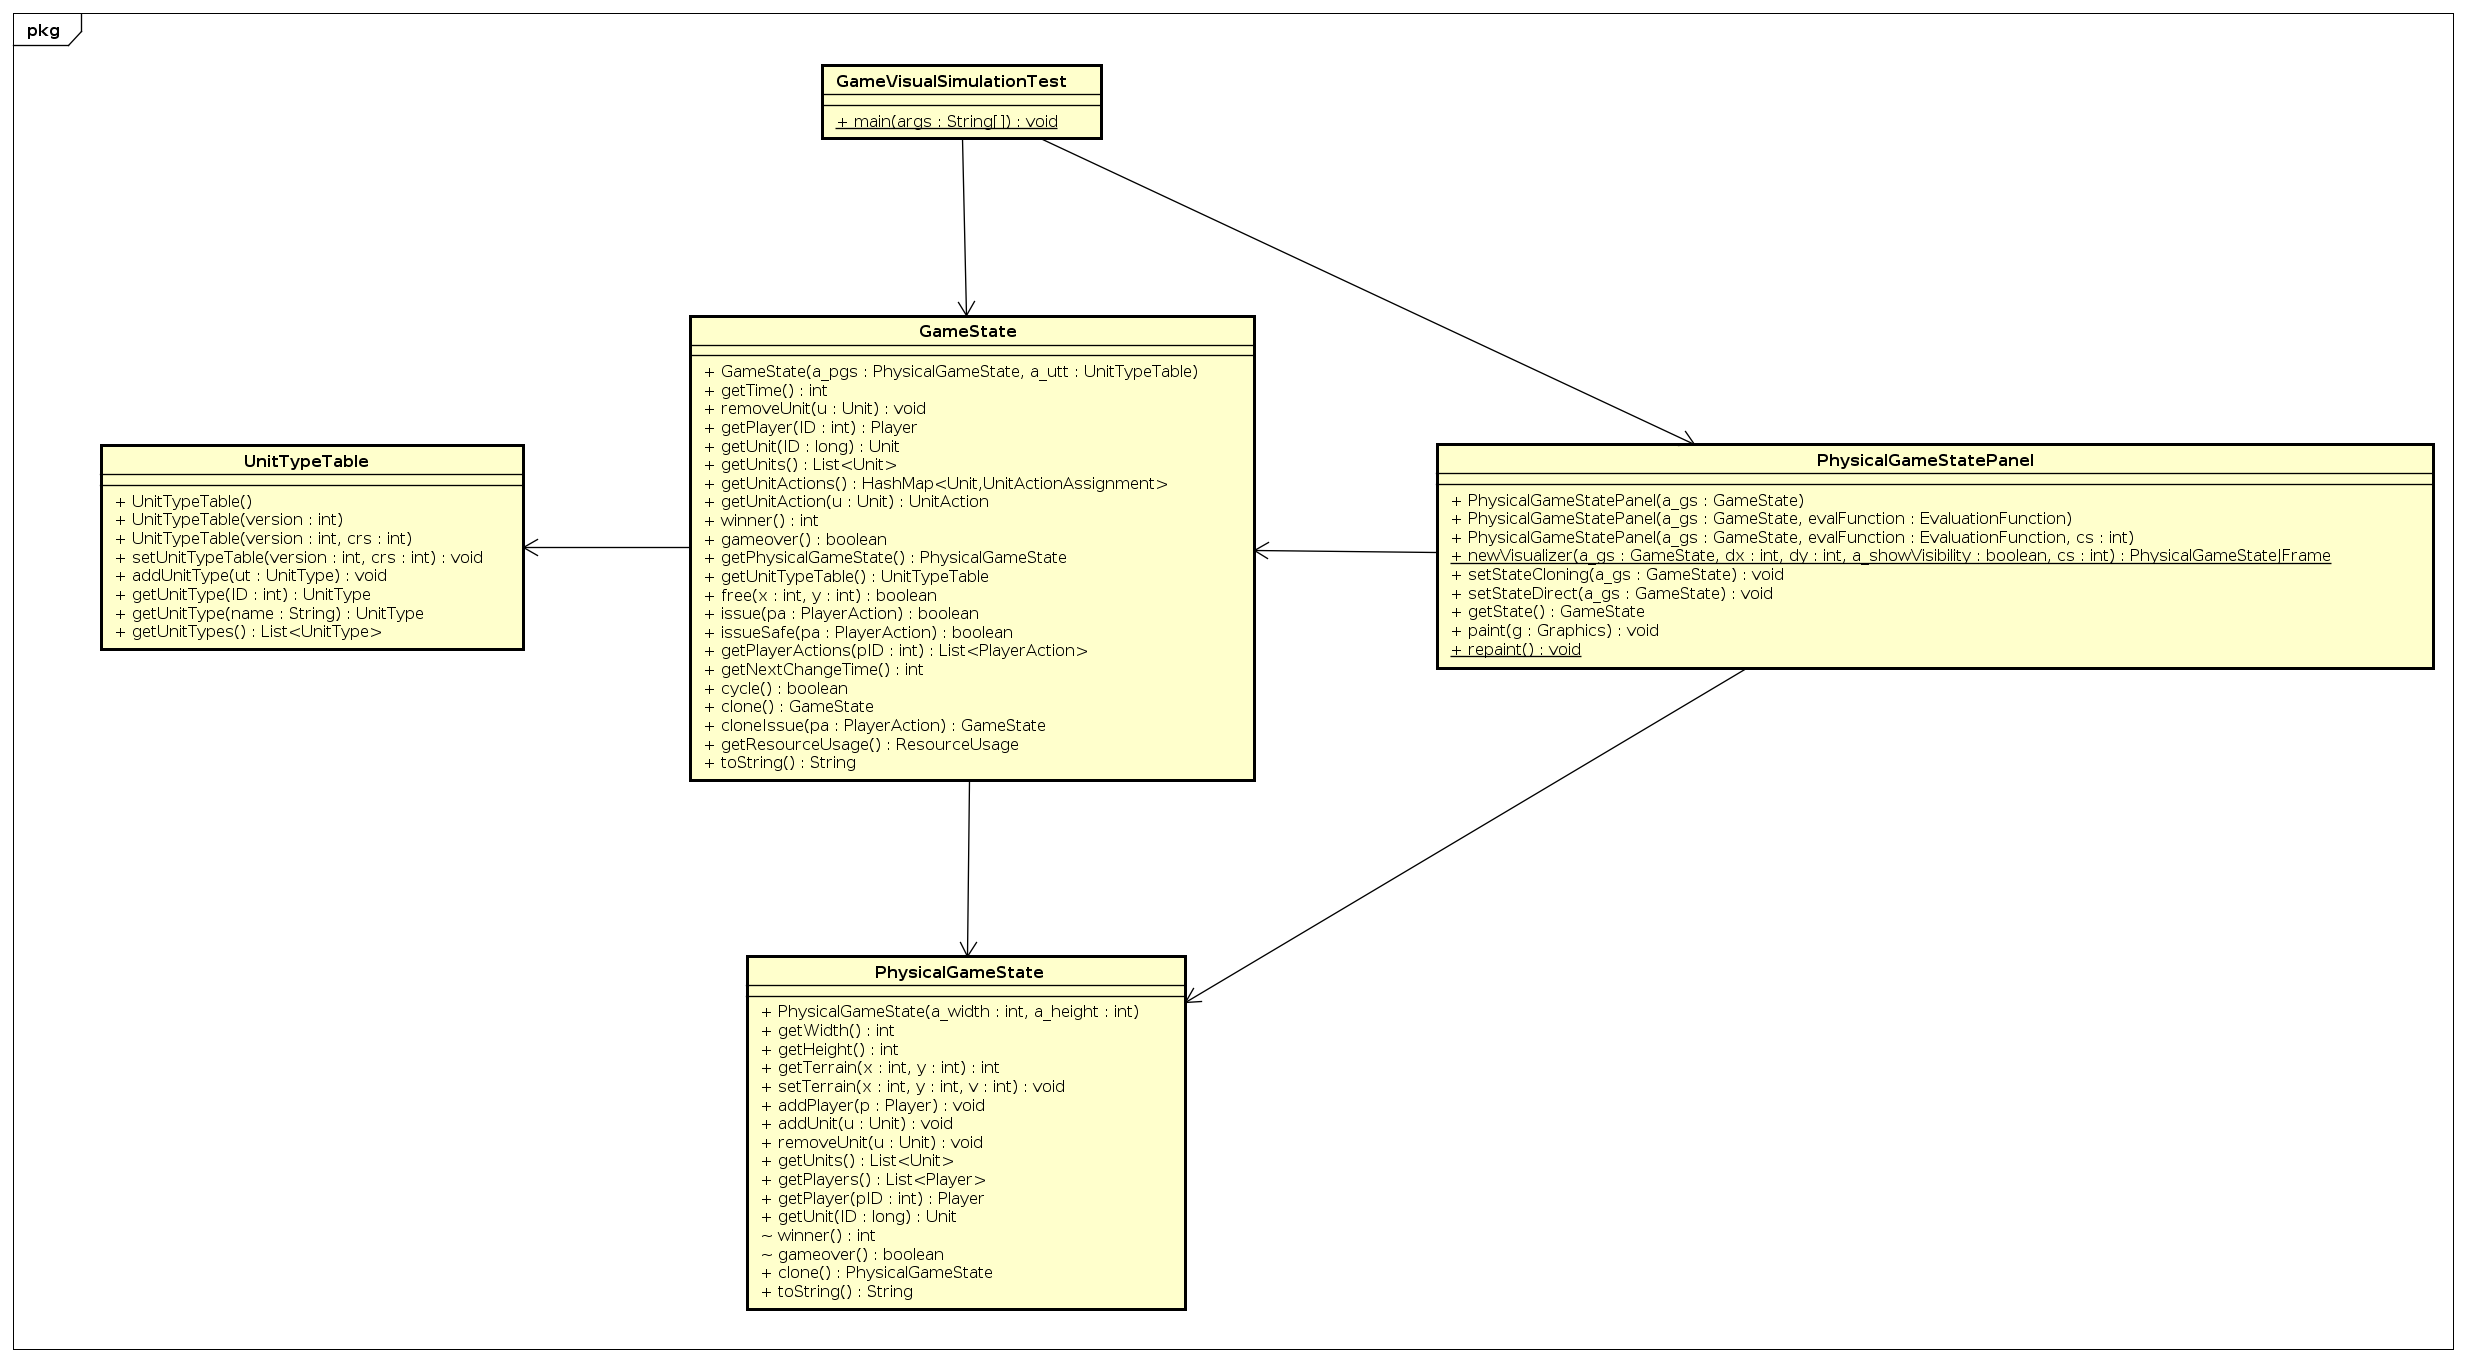
\includegraphics[width=1\textwidth]{fig/classes.png}
	\caption{Classes do MicroRTS}
	\label{fig:classes}
\end{figure} 

O MicroRTS fornece uma camada de abstração para que se possa utilizar as unidades, sem precisar ter conhecimento de como elas estão estruturadas. 
Essa camada se chama \textit{AbstractionLayerAI}. 
Ela apresenta métodos para treinar unidades, construir edificações, coletar recursos, atacar, e movimentar as unidades. 
Esta camada oferece todos os recursos necessários para que seja implementado uma IA.

Toda a IA que for implementada no MicroRTS deve conter o método $\mathit{getAction}$.
Este método é responsável por determinar qual ação deve ser realizada pela IA em determinado momento do jogo.
Cada IA pode assumir o lugar de um jogador no MicroRTS. 
A classe \textit{GameVisualSimulation}, que é responsável por gerenciar a simulação, inicializa os jogadores e a cada período de tempo chama o método realizar as ações dos jogadores.
A Figura~\ref{fig:sequencia} ilustra o diagrama de sequência do funcionamento da classe \textit{GameVisualSimulation}. 

O algoritmo Algoritmo~\ref{alg:jogo} apresenta o pseudo código da classe. 
A classe primeiro obtém as instâncias dos objetos necessários para a simulação do jogo, esse processo está representado a partir da linha~\ref{alg:jogo:instancia} até a linha~\ref{alg:jogo:instanciaend}.
A linha~\ref{alg:jogo:desenha} é onde o algoritmo chama a classe da interface gráfica para desenhar a tela do jogo.
Após isso, o jogo entra em um laço para que os jogadores façam suas jogadas. As linhas~\ref{alg:jogo:action1} e \ref{alg:jogo:action2} são onde os jogadores escolhem qual as suas jogadas.
Nas linhas~\ref{alg:jogo:issue1} e \ref{alg:jogo:issue2} as jogadas são testadas para que não haja nenhuma violação quanto as restrições do jogo.
Na linha~\ref{alg:jogo:gameover} é responsável por determinar se o jogo não acabou.
A linha~\ref{alg:jogo:repaint} desenha a tela novamente com as jogadas executadas.
Assim o laço da linha~\ref{alg:jogo:while} é executado até que o jogo termine com algum vencedor, ou quando o tempo de simulação acabar.

\begin{algorithm}
	\caption{Pseudo código da classe \textit{GameVisualSimulation}.}
	\label{alg:jogo}
	\begin{algorithmic}[1]		
		\Function {main}{$String[]$}
		\State $utt = UnitTypeTable()$ \label{alg:jogo:instancia}
		\State $pgs = PhysicalGameState()$
		\State $gs = GameState(pgs, utt)$
		\State $player1 = Player1()$
		\State $player2 = Player2()$ \label{alg:jogo:instanciaend}
		\State $drawScreen()$  \label{alg:jogo:desenha}
		\While{$!gameover() || endTime()$} \label{alg:jogo:while}
			\State $action1 = player1.getAction()$ \label{alg:jogo:action1}
			\State $action2 = player2.getAction()$ \label{alg:jogo:action2}
			\State $issueSafe(action1)$ \label{alg:jogo:issue1}
			\State $issueSafe(action2)$ \label{alg:jogo:issue2}
			\State $gameover = gs.cycle()$ \label{alg:jogo:gameover} 
			\State $repaintScreen()$ \label{alg:jogo:repaint}
		\EndWhile
		\EndFunction
	\end{algorithmic}
\end{algorithm}

\begin{figure}[ht]
	\centering
	\frm[inline]{Está em PDF, mas ainda não é vetorial.}
	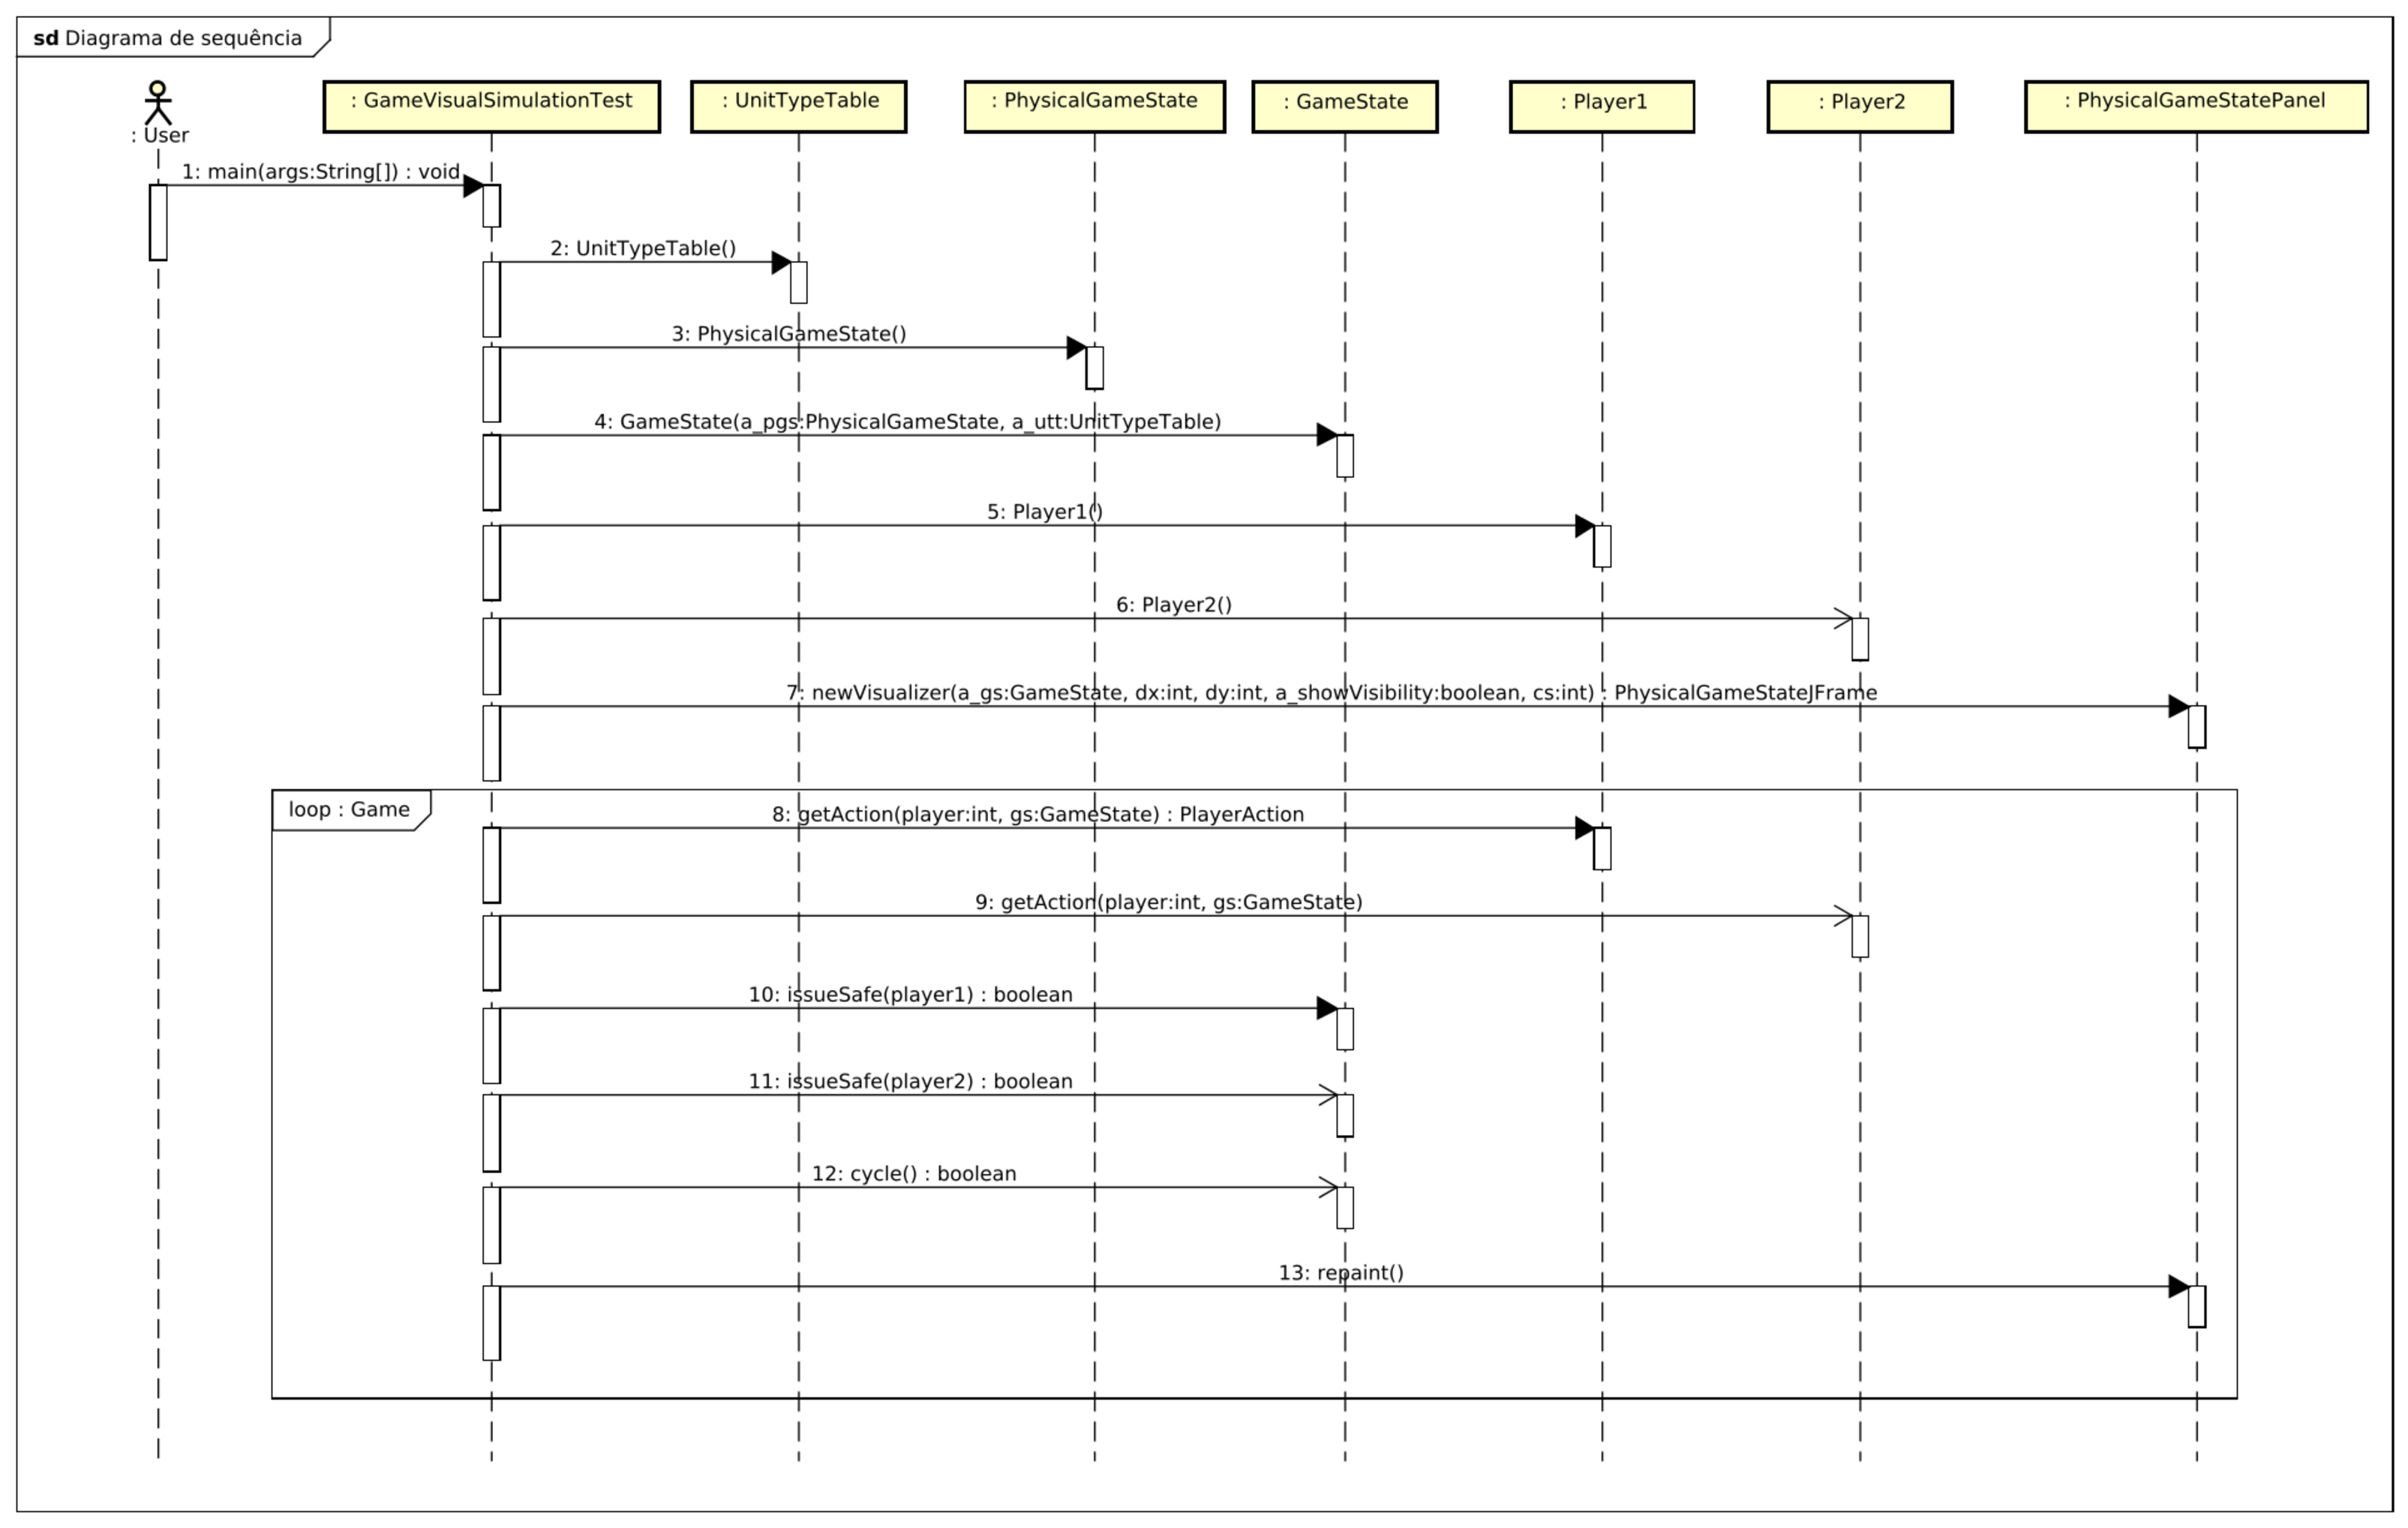
\includegraphics[width=1\textwidth]{fig/diagramaSequencia.pdf}
	\caption{Diagrama de sequência}
	\label{fig:sequencia}
\end{figure}

\subsection{Técnicas de IA}

O MicroRTS possui algumas técnicas de IA já implementadas.
Algumas destas técnicas simulam algum comportamento dentro do jogo, sem ter um algoritmo de IA, essas técnicas são chamadas de estratégias Hard-Coded. 
Dentro das estratégias Hard-Coded, existem duas técnicas que são baseadas em executar movimentos aleatórios, elas são chamadas de RandomAI e RandomBiasedAI.
A RandomAI executa movimentos totalmente aleatórios.
Já a RandomBiasedAI executa movimentos aleatórios mas com probabilidade maior de realizar movimentos de ataque, ou extração de recurso, ou criação de tropas.
Ainda dentre as estratégias Hard-Coded, existem técnicas que utilizam uma mesma dinâmica. 
Elas utilizam um \textit{worker} para extrair recursos, e treinam unidades de ataque para atacar. 
Essas técnicas se diferenciam no tipo de unidade de ataque que é criado. 
As técnicas são chamadas de LightRush, HeavyRush, e RangedRush, elas utilizam as unidades \textit{light}, \textit{heavy}, e \text{ranged}, respectivamente.
A ultima técnica deste tipo de categoria é chamada de WorkerRush, ela consiste ter um \textit{worker} para realizar a extração de recursos, mas ao invés de treinar unidades de ataque, ela treina outros \textit{workers} para realizar os ataques, isso faz com que a técnica consiga criar muitas unidades de maneira rápida.

Outras técnicas utilizam algum algoritmo de IA para decidir qual ação deve ser realizada.
Como é o caso das estratégias Minimax, Monte Carlo, e Portfolio Search.
A estratégia de Minimax utiliza o algoritmo de minimax para uma determinada profundidade. A profundidade não é em relação aos turnos, como no algoritmo comum de minimax, mas sim ao tempo disponível para tomar um decisão.
A estratégia de Monte Carlo verifica todas as ações possíveis para o estado, e simula jogos aleatórios para aquela jogada até um determinado tempo. Uma heurística é utilizada para determinar qual foi a ação que obteve o melhor valor.
Já estratégia de Portfolio Search possui um conjunto de estratégia e utiliza um algoritmo de busca para decidir qual a melhor estratégia para ser usada em determinado momento. O conjunto é composto pelas estratégias Hard-Coded.

\section{Java Simple Hierarchical Ordered Planner 2}\label{sec:jshop}
		
Java Simple Hierarchical Ordered Planner 2 (JSHOP2)~\cite{ilghami2006documentation} é um sistema de planejamento independente de domínio baseado em HTN. O JSHOP2 foi desenvolvido em Java por Dana Nau e sua equipe de pesquisa. 

O JSHOP2 recebe como entrada uma descrição do domínio e um problema de planejamento. 
A descrição do domínio contém a formalização das ações dos agentes, as tarefas e métodos que as decompõem.
O planejador realiza a geração do plano decompondo os métodos até que só restem tarefas primitivas. Na descrição do domínio as tarefas primitivas são descrita como operadores. Na descrição do domínio os operadores são compostos por um nome de operador, uma lista de precondições que deve ser verdadeira para a execução do operador, uma lista de elementos que serão removidos do estado, e uma lista de elementos que serão adicionados ao estado, um exemplo de operador é apresentado a seguir:

\lstset{style=codeStyle}
\begin{lstlisting}[language=lisp]
	(:operator (!move ?from ?to) 
		((at ?from)) 
		((at ?from))
		((at ?to))
	)
\end{lstlisting}

Os métodos são utilizados para decompor tarefas de alto nível para níveis mais baixos. No JSHOP2 os métodos são identificados por um nome de método, que é único para cada método. Dentro de um método há uma lista de precondições, e uma lista de tarefas, que podem ser primitivas ou não primitivas, para quantos casos forem necessário. Por exemplo, o problema de ir de um local para outro, se o local destino tem um caminho para o local origem, é possível se locomover para o local, mas se não houver caminho é preciso ir para outra cidade que tenha caminho para o local destino. Este exemplo pode ser visto abaixo:

\lstset{style=codeStyle}
\begin{lstlisting}[language=lisp]
	(:method (travel ?from ?to)
		((at ?from) (path ?from ?to))
		((!move ?from ?to))
		
		((not (path ?from ?to)) (path ?from ?somewhere))
		((!move ?from ?somewhere) (travel ?somewhere ?to))
	)
\end{lstlisting}

O domínio completo começa com o nome do domínio e em seguida os operadores e métodos descritos. O domínio completo exemplo ficaria assim: 

\lstset{style=codeStyle}
\begin{lstlisting}[language=lisp]
(defdomain move
	(
		(:operator (!move ?from ?to) 
			((at ?from)) 
			((at ?from))
			((at ?to))
		)
	
		(:method (travel ?from ?to)
			((at ?from) (path ?from ?to))
			((!move ?from ?to))
		
			((not (path ?from ?to)) (path ?from ?somewhere))
			((!move ?from ?somewhere) (travel ?somewhere ?to))
		)    
	)
)
\end{lstlisting}

O problema de planejamento contém as informações do estado do ambiente e qual é o objetivo do agente. 
O estado do ambiente é composto por predicados que são usados nos métodos e operadores, como no exemplo $at ?x$ e $path ?a ?b$. E o objetivo do agente é um método do domínio, no exemplo $travel ?from ?to$. Um possível problema de planejamento para o exemplo pode ser o apresentado abaixo:


\begin{lstlisting}[language=lisp]
(defproblem problem move
	( 
		(path PortoAlegre Charqueadas)
		(path Charqueadas SaoJeronimo)
		(at PortoAlegre)
	)
	
	(
		(travel PortoAlegre SaoJeronimo)
	)
)
\end{lstlisting}

O JSHOP2 gera duas classes java, uma representando o domínio, e a outra representando o problema.
A classe do problema gera o plano, utilizando as informações da classe da descrição do domínio.
Uma vez que o domínio esteja consolidado não é preciso gerar a classe do domínio novamente. A classe do problema deve mudar dependendo do estado do ambiente.  
O plano gerado para o exemplo acima é o seguinte:

\begin{lstlisting}[language=lisp]
[Plan cost: 2.0

(!move portoalegre charqueadas)
(!move charqueadas saojeronimo)
--------------------
]
\end{lstlisting}

O plano indica o custo do plano, junto com os operadores em ordem que devem ser executados para que o objetivo seja alcançado. 
Caso existam mais planos que levem ao mesmo objetivo, o JSHOP2 apresenta os planos na mesma estrutura.

Este capítulo apresenta todos os requisitos necessários para a implementação do algoritmo de AHTN.
A Seção~\ref{sec:microrts} apresenta como é o funcionamento do MicroRTS, e em qual parte do jogo o algoritmo pode ser implementado.
Na Seção~\ref{sec:jshop} é apresentado o planejador HTN que será utilizado para gerar os planos usados no algoritmo. 
No próximo capítulo é apresentado como foi feita a modelagem do domínio, a implementação do algoritmo de AHTN no MicroRTS, e como foi feita a tradução do cenário do jogo para um problema de planejamento.


%!TEX root = volumeFinal.tex 

\chapter{\label{chap:impl}Implementação}

A implementação do algoritmo de AHTN dentro do MicroRTS foi feita em duas etapas.
Primeiro foi feita a modelagem do domínio e criada a heurística que define o valor de utilidade para os estados.
Na segunda etapa foi acoplado o JSHOP2 com o MicroRTS, e logo após foi feita a implementação do algoritmo AHTN.

\section{Modelagem do domínio}

Antes de realizar a implementação do algoritmo de AHTN é preciso criar um domínio de planejamento. 
O domínio de planejamento serve para que o JSHOP2 consiga gerar os planos que serão usados pelo algoritmo.

A modelagem do domínio inicia com a especificação de qual estratégia o domínio vai adotar.
O domínio é pensado em uma situação de jogo, onde o jogador quer treinar uma unidade de ataque para destruir o seu adversário.
Sendo assim, o jogador precisa de um quartel para treinar as unidades e uma base para os recursos serem guardados.
O domínio tem apenas uma de cada edificação.
Apenas um \textit{worker} é utilizado, responsável pela extração dos recursos e construção das edificações.
Quando o quartel está criado e há recursos para treinamento de um unidade de ataque, a unidade \textit{ranged} é criada.
Assim que uma unidade de ataque estiver pronta, ela é enviada para atacar o adversário.
Apenas quando a unidade \textit{ranged} é destruída outra unidade é criada.
Todos os mapas testados iniciam com uma base, pois a base é necessária para treinar \textit{workers} e para guardar os recursos.  

A modelagem do domínio começa pela descrição dos operadores.
Cada ação que pode ser executada dentro do jogo é descrita como um operador no domínio.
Por exemplo, as ações de construir um quartel e coletar recursos são transformadas nos operadores $!buildbarrack$ e $!getresource$, respectivamente.
Já os métodos servem para determinar ações de mais alto nível e devem respeitar a estratégia definida.
Por exemplo, no domínio apenas um quartel é construído, então o método deve ter uma precondição para verificar se existe outro quartel no jogo, caso não tenha é preciso checar se há recursos suficientes para construir. 
Cada método pode encadear a chamada de outros métodos do domínio.
Isso acontece pois pode ser necessário realizar outra ação antes de conseguir realizar a ação que o método está tentando fazer.
Por exemplo, é necessário um quartel para treinar uma unidade de ataque, portanto quando o método de treinar unidade é chamado, ele verifica se há um quartel e chama o método de construir o quartel se não existe um.

Para ganhar o jogo é preciso atacar o adversário, por essa razão o método utilizado como objetivo no problema de planejamento é o $ataqueranged$.
Esse método desencadeia todas as outras chamadas de método dependendo do estado do ambiente.
No Apêndice~\ref{ap:estra1} está a descrição deste domínio, que é chamado de domínio 1.

O domínio 1 treina apenas uma unidade de ataque, o que acaba limitando o poder de ataque da estratégia.
Para tentar solucionar esse problema, outro domínio foi modelado.
Esse domínio tem a mesma estratégia do domínio anterior, com a diferença de que mais de uma unidade de ataque é criada.
Assim, enquanto uma unidade está atacando, outra pode estar sendo treinada.
No Apêndice~\ref{ap:estra2} está a descrição deste domínio, que é chamado de domínio 2.


\section{Heurística}

O algoritmo de AHTN requer uma função de avaliação para determinar o valor de utilidade para cada estado do jogo. Essa função utiliza uma heurística para determinar o valor de utilidade.
Foram criadas duas heurísticas.
A primeira leva em consideração apenas as unidades do jogador.
Quanto maior o número de unidades disponíveis no ambiente melhor a função de avaliação do estado.
As unidades são ponderadas pelo custo de treinamento ou de construção, isso é necessário porque o custo de treinamento ou construção de cada unidade é diferente.
A Equação~\ref{eq:heu1} ilustra a fórmula para essa heurística.

\begin{equation}
\label{eq:heu1}	
avaliacao(s) =  (1*worker) + (5 * quartel) + (10 * base) + (2 * unidadesDeAtaque)
\end{equation}

O problema dessa heurística é que as unidades do adversário não estão sendo levadas em consideração.
Se um jogador tem o dobro de unidades que o outro, isso é um indício que ele está ganhando o jogo.
Para resolver o problema outra heurística foi criada.
Essa heurística utiliza a mesma maneira de calcular da Equação~\ref{eq:heu1}, mas também calcula o mesmo valor para as unidades do adversário. 
O valor das unidades que o jogador possui é subtraído do valor das unidades do adversário. 
Assim em um cenário onde o jogo está com mais tropas a favor, o valor de utilidade é positivo e caso o contrário negativo.
Esta heurística foi a escolhida para ser utilizada na implementação.

Se um jogador não tem uma base nem recursos para construir uma, o jogo está perdido pois a base é necessária para armazenar os recursos. 
Nesse caso, as duas heurísticas retornam um valor negativo, indicando o fim do jogo. 

\section{Implementação}

\subsection{Ações do MicroRTS}

Antes de iniciar a implementação do algoritmo de AHTN, é preciso criar os métodos em Java que executam as ações dentro do MicroRTS.
A camada de abstração fornece as classes responsáveis por exercer essas funções, mas ainda assim é preciso informar qual unidade o método está chamando.
Para isso foram criados 6 métodos que utilizam as classes da camada.
Cada método fica responsável por apenas uma ação dentro do jogo.
Os métodos realizam as seguintes ações: construir uma base, construir um quartel, treinar um \textit{worker}, fazer um \textit{worker} coleta recursos, treinar unidade de ataque, e fazer uma unidade de ataque procura unidades adversárias para atacar.

\subsection{Geração dos planos}

O algoritmo de AHTN decompõe todas as possibilidades de plano para um objetivo com determinada configuração do jogo.
Para gerar os planos foi utilizado o planejador JSHOP2.
O JSHOP2 gera duas classes java, uma representando o domínio e outra representando o problema.
A classe do domínio gerada traduz as informações relativas aos métodos, operadores, e as ligações entre eles, para estruturas de dados do Java.
Já a classe do problema contém o estado do ambiente e as tarefas que desejam ser alcançadas.
A classe do problema gera o plano utilizando as estruturas da classe do domínio.

A classe que representa o domínio não precisa ser alterada, pois são sempre os mesmo operadores e métodos que são utilizados para gerar o plano.
Mas o problema muda a cada nova configuração do ambiente.
Nesse caso a classe do problema deve ser alterada para que represente um novo estado.
Essa mudança foi feita alterando a classe java originada pelo JSHOP2. 
A mudança consiste em gerar novos predicados a cada nova configuração.
Para isso foi preciso uma análise de como é guardado internamente cada um dos componentes do problema de planejamento na classe do JSHOP2.
A partir dessa análise houve o mapeamento dos estados do jogo para os predicados do problema.

Uma classe chamada de $EstadoDoJogo$ foi criada para representar o estado em que o jogo está em determinado momento.
A classe contém informações das unidades que cada jogador tem em determinada configuração do jogo, podendo ser alterada caso alguma ação seja executada.
A cada novo estado é gerado um conjunto de predicados que representam o jogo, para que o planejador consiga gerar os planos possíveis de serem feitos.

A Figura~\ref{fig:planos} ilustra a comunicação necessária para geração dos planos.
A geração de um plano é feita a partir da chamada do método \texttt{getPlanos}.
Para isso, é necessário informar qual o estado do jogo.
A classe do problema, gerada pelo JSHOP2, pega as informações do domínio e gera os planos a partir do estado do jogo informado.
Por fim, os planos gerados são retornados para a classe dentro do MicroRTS.

\begin{figure}[ht]
	\centering
	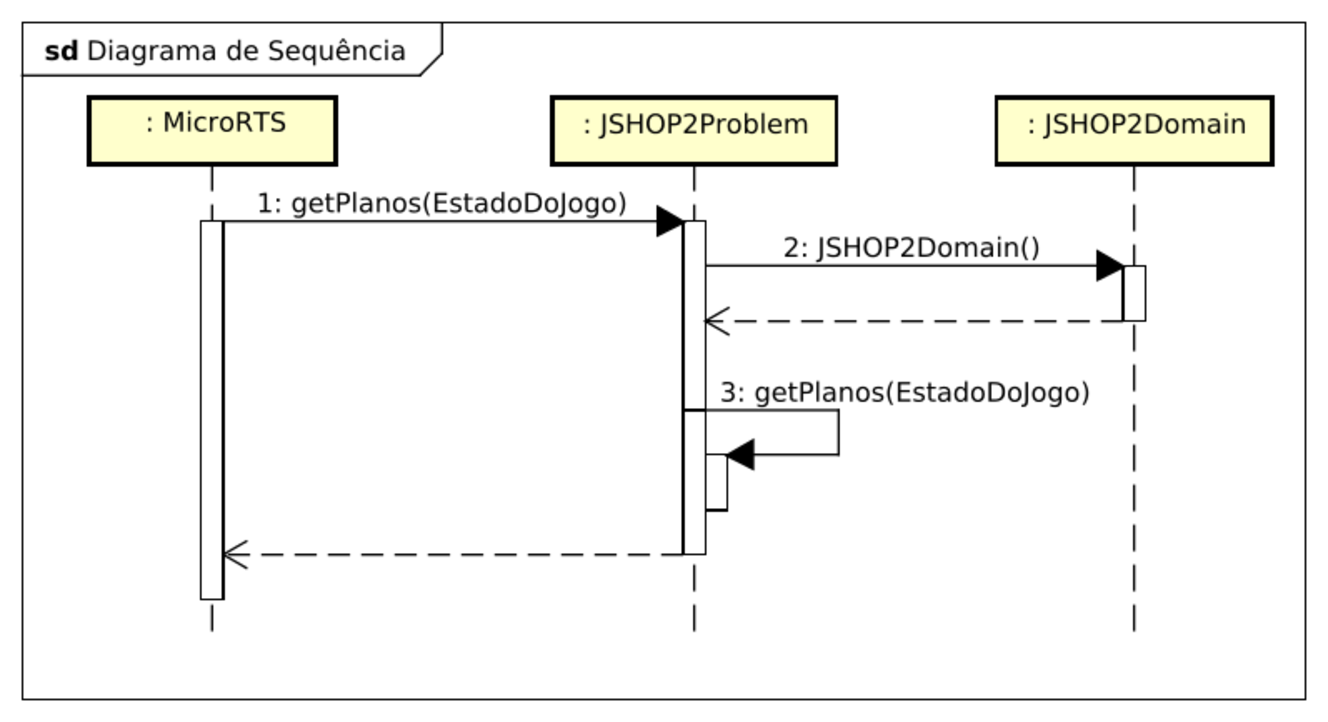
\includegraphics[width=0.9\textwidth]{fig/gerarPlano.pdf}
	\caption{Comunicação entre o MicroRTS e as classes do JSHOP2}
	\label{fig:planos}
\end{figure}

\subsection{Algoritmo de AHTN}

Para que o MicroRTS reconheça uma IA, ela deve ter o método $\mathit{getAction}$ implementado.
Quando este método é invocado, a técnica deve realizar a sua operação e retornar qual movimento deve ser realizado.
Sendo assim, a classe que implementa o algoritmo de AHTN deve utilizar este método para retornar à ação encontrada pelo algoritmo de AHTN.
O algoritmo de AHTN implementado seguiu o padrão do algoritmo apresentado na Seção~\ref{alg:ahtn}, mas com algumas alterações.

O JSHOP2 gera os planos apenas com os operadores utilizados para alcançar o objetivo.
Com isso, o plano gerado não tem a informação de quais métodos foram utilizados para chegar aos operadores.
Neste caso, o plano contém os operadores ordenados que chegam ao objetivo.
No algoritmo de AHTN original o plano vai sendo decomposto através dos métodos à medida que a árvore das jogadas está expandindo e só realiza a troca de perspectiva entre \textsc{Max} e \textsc{Min} quando há uma tarefa primitiva a ser executada.
No algoritmo de AHTN implementado há uma pequena diferença do algoritmo original.
No algoritmo implementado sempre acontece a troca de perspectiva a cada rodada.
A troca de perspectiva é feita para cada plano que é gerado a partir do estado do jogo.
O Algoritmo~\ref{alg:meuahtn} ilustra o pseudo código do algoritmo de AHTN implementado.

O algoritmo recebe um estado, representando qual a configuração do ambiente, um plano para a perspectiva \textsc{Max}, um plano para a perspectiva \textsc{Min}, e uma profundidade.
A Linha~\ref{alg:meuahtn:terminal} verifica se o estado é uma configuração de final de jogo, ou ainda se a profundidade configurada foi atingida.
Caso uma das duas coisas aconteça, o algoritmo retorna o plano de cada perspectiva, e também a função de avaliação para a configuração em que o jogo se encontra.

O algoritmo avança caso não haja uma configuração de final de jogo.
Na linha~\ref{alg:meuahtn:nexaction} o algoritmo aplica a próxima ação primitiva do plano no estado.
Neste ponto, o jogador realiza uma ação no estado.
Após alterar o estado, o algoritmo gera todos os planos para \textsc{Min} a partir do novo estado e realiza a chamada para o método $\mathit{AHTNMin}$.
O método de $\mathit{AHTNMin}$ realiza as mesmas operações que o método de $\mathit{AHTNMax}$ mas com a perspectiva de \textsc{Min}.
Seguindo, na linha~\ref{alg:meuahtn:avali}, o algoritmo verifica qual dos planos obteve a melhor função de avaliação. 
Com isso, o algoritmo decide qual a melhor opção de plano.
O melhor plano é retornado na linha~\ref{alg:meuahtn:retorno}.


\begin{algorithm}[ht]
	\caption{Pseudo código do algoritmo de AHTN implementado.}
	\label{alg:meuahtn}
 	\begin{algorithmic}[1]		
 		\Function {ATHNMax}{$estado, planoMax, planoMin, deph$}
	 		\If {$terminal(estado) \vee d \leq 0$} \label{alg:meuahtn:terminal}
		 		\State	\Return $(planoMax, planoMin, avaliacao(estado))$
	 		\EndIf
	 		\State {$nextAction(planoMax)$} \label{alg:meuahtn:nexaction}
	 		\State $(Pmax', Pmin', ev') = \perp, \perp, -\infty$
			\ForAll{$plano \in getPlanos(estado)$} \label{alg:meuahtn:for}
		 		\State $(Pmax, Pmin, ev) = \Call{AHTNMin}{(estado, planoMax, planoMin, deph-1)}$ \label{alg:meuahtn:ahtnmin}
			 	\If {$ev' > ev$} \label{alg:meuahtn:avali}
					\State $(Pmax', Pmin', ev') = (Pmax, Pmin, ev)$
				\EndIf		 		 		
		 	\EndFor
		 	\State \Return $(Pmax', Pmin', ev')$ \label{alg:meuahtn:retorno}
 		\EndFunction
 	\end{algorithmic}
 \end{algorithm}
 
 
O método $\mathit{getAction}$ é responsável pela chamada do algoritmo de AHTN. 
Ele realiza a chamada para o método de $\mathit{AHTNMax}$ para todos os planos possíveis no estado atual.
O retorno indica qual plano tem a melhor função de avaliação.
A primeira ação do plano com a melhor função de avaliação é a escolhida para ser executada. 

O método $\mathit{getAction}$ é chamado a todo ciclo para decidir qual jogada deve ser realizada.
As ações geralmente não são realizadas em um ciclo.
Por exemplo, treinar uma unidade leva alguns ciclos.
Assim o algoritmo gera muitas vezes a mesma ação.
Foi definido um tempo de 50 ciclos para gerar uma nova ação.
Com isso o número de ações geradas repetidamente foi reduzido.


%!TEX root = volumeFinal.tex 

\chapter{\label{chap:results}Resultados - Avaliação de Desempenho}

Foram utilizados três mapas para avaliar o desempenho do algoritmo.
A avaliação dos resultados está divida por mapa.
Em cada mapa é possível jogar em dois lados.
O lado azul começa o jogo na parte superior do mapa, e o lado vermelho começa na parte inferior.
Em cada mapa é avaliado a porcentagem de vitórias para cada domínio.
Os adversários, utilizados para testar o algoritmo, são as técnicas presentes no MicroRTS apresentadas na Seção~\ref{sec:tecn}.
Cada adversário foi utilizado dez vezes em cada mapa, e em cada lado do jogo.

\frm[inline]{As avaliações estão um pouco superficiais. Por que o portfolio ganha sempre em algumas? O quanto influi a tua descrição de domínio?}
\section{Mapa 1}

No primeiro mapa, cada jogador inicia com uma base, um \textit{worker} e dois recursos próximos a sua base.
O mapa é formado por 16x16 posições.
O lado azul e o lado vermelho tem a mesma formação dos componentes iniciais.
A Figura~\ref{fig:mapa16x16} ilustra a tela do jogo com a configuração inicial do mapa.

\begin{figure}[ht]
	\centering
	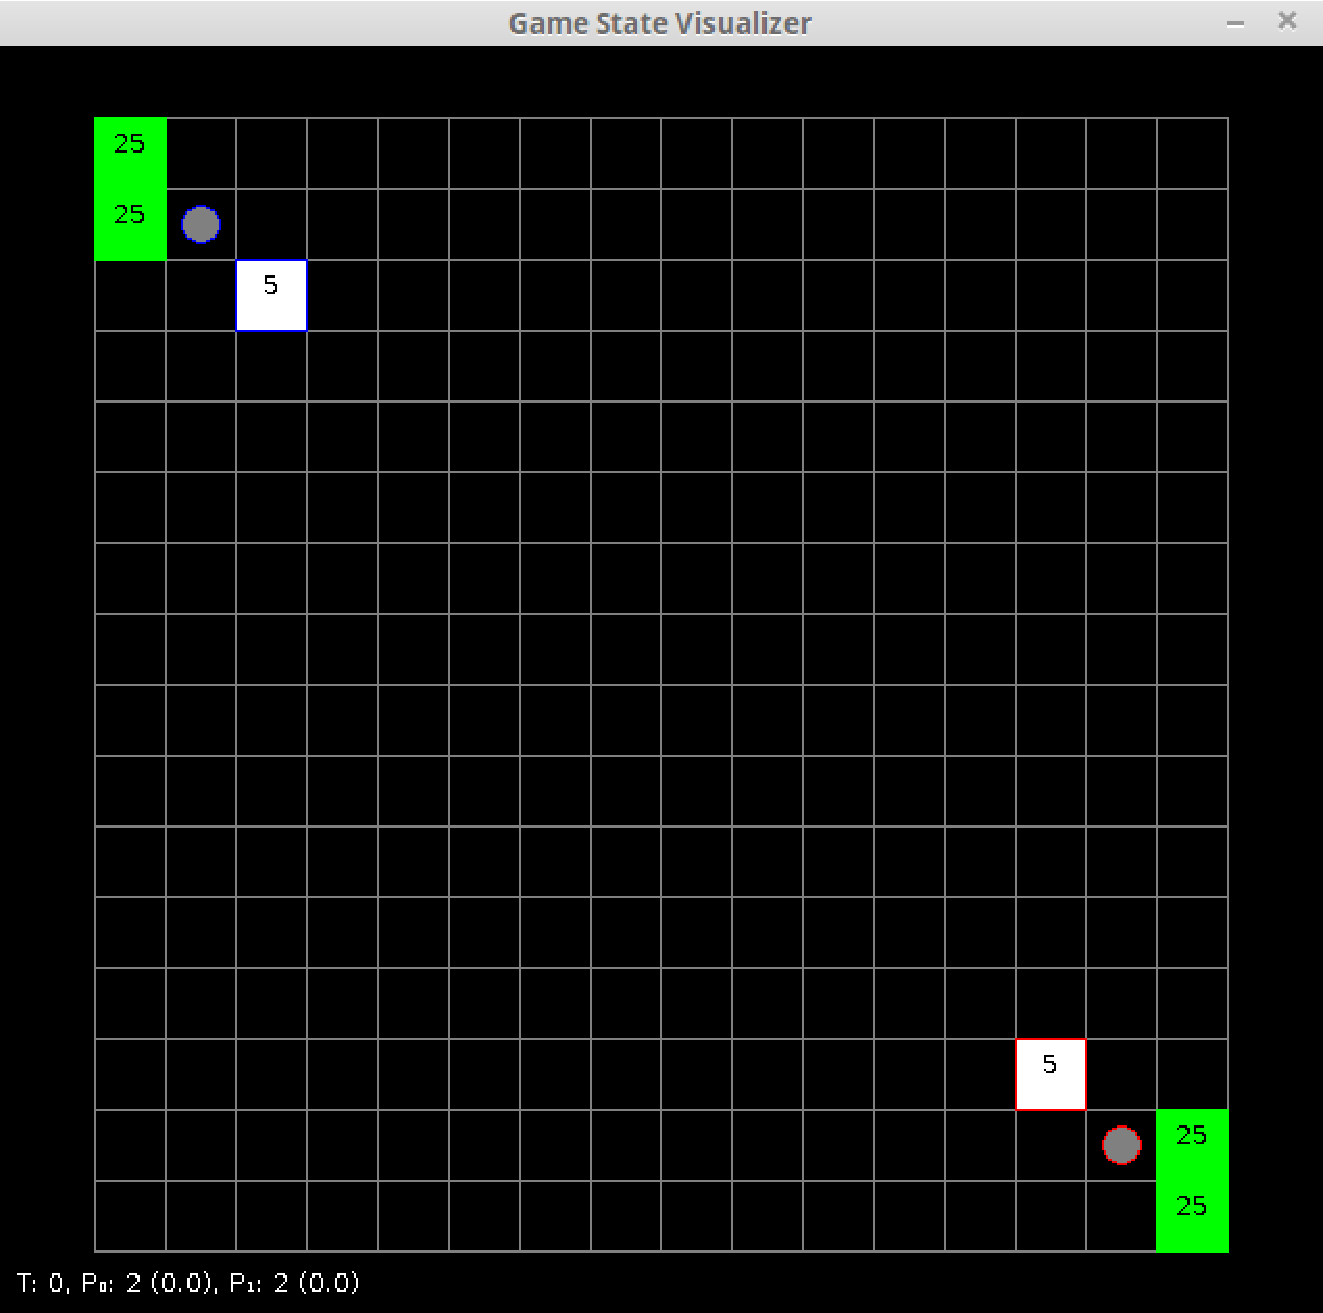
\includegraphics[width=.5\textwidth]{fig/map16x16.pdf}
	\caption{Configuração inicial do mapa 1.}
	\label{fig:mapa16x16}
\end{figure}


A Tabela~\ref{tab:mapa1} ilustra os resultados obtidos com o algoritmo de AHTN contra as técnicas do MicroRTS.
Quando o domínio 1 é executado do lado vermelho, ocorre a criação de duas unidades de ataque ao invés de uma.
Isso ocorre porque o tempo de criação da unidade é maior que o da geração de outra ação do algoritmo.
Quando o algoritmo é invocado novamente, ele não tem conhecimento da unidade que está prestes a ser criada, e assim ocorre a duplicação dessa outra unidade.
O tempo de espera para que o algoritmo gere outra ação foi alterado para tentar remover esse problema.
Mas com um tempo maior, as outras ações eram afetadas, e o algoritmo se torna menos vitorioso.

\begin{table}[ht]
	\centering
	\caption{Porcentagem de vitórias do AHTN no mapa 1.}
	\label{tab:mapa1}
	\begin{tabular}{|c|cc|cc|}
		\hline
		\textbf{}           & \multicolumn{2}{c|}{\textbf{Domínio 1}}  & \multicolumn{2}{c|}{\textbf{Domínio 2}}  \\ \hline
		\textbf{Adversário} & \textbf{Lado Azul} & \textbf{Lado Vermelho} & \textbf{Lado Azul} & \textbf{Lado Vermelho} \\ \hline
		RandomIA            & 100\%              & 100\%                  & 100\%              & 100\%                  \\ \hline
		RandomBiasedIA      & 80\%               & 100\%                  & 100\%              & 100\%                  \\ \hline
		RangedRush          & 0\%                & 100\%                  & 100\%              & 100\%                  \\ \hline
		HeavyRush           & 0\%                & 100\%                  & 0\%                & 100\%                  \\ \hline
		LightRush           & 0\%                & 100\%                  & 0\%                & 100\%                  \\ \hline
		WorkerRush          & 0\%                & 0\%                    & 0\%                & 0\%                    \\ \hline
		MonteCarlo          & 60\%               & 80\%                   & 100\%              & 100\%                  \\ \hline
		Minimax             & 100\%              & 100\%                  & 100\%              & 100\%                  \\ \hline
		Portfolio           & 0\%                & 0\%                    & 0\%                & 0\%                    \\ \hline
	\end{tabular}
\end{table}

A partir dos dados da tabela é possível observar que há um ganho do lado vermelho em relação ao azul nos dois domínios. 
No domínio 1 o motivo foi a duplicação da unidade.
Já no domínio 2, a ação de construir o quartel, gerada pela camada de abstração do MicroRTS, encontra uma posição mais favorável do lado vermelho.
Fazendo com que o lado vermelho tenha uma melhor fluidez na hora da criação das tropas.
O domínio 2 consegue melhores resultados do que o domínio 1.
Adversários que não são vencidos no lado azul passam a ser vencidos com o segundo domínio, e os resultados do lado vermelho são consolidados.

\section{Mapa 2}

Neste mapa, cada jogador inicia com uma base, um \textit{worker}, um quartel e um recurso perto de sua base.
O mapa é composto por 8x8 posições.
O quartel está construído no limite superior do mapa para o jogador azul, e no limite inferior do mapa para o jogador vermelho.
A Figura~\ref{fig:mapa8x8quartel} ilustra a tela do jogo com a configuração inicial do mapa.

\begin{figure}[ht]
	\centering
	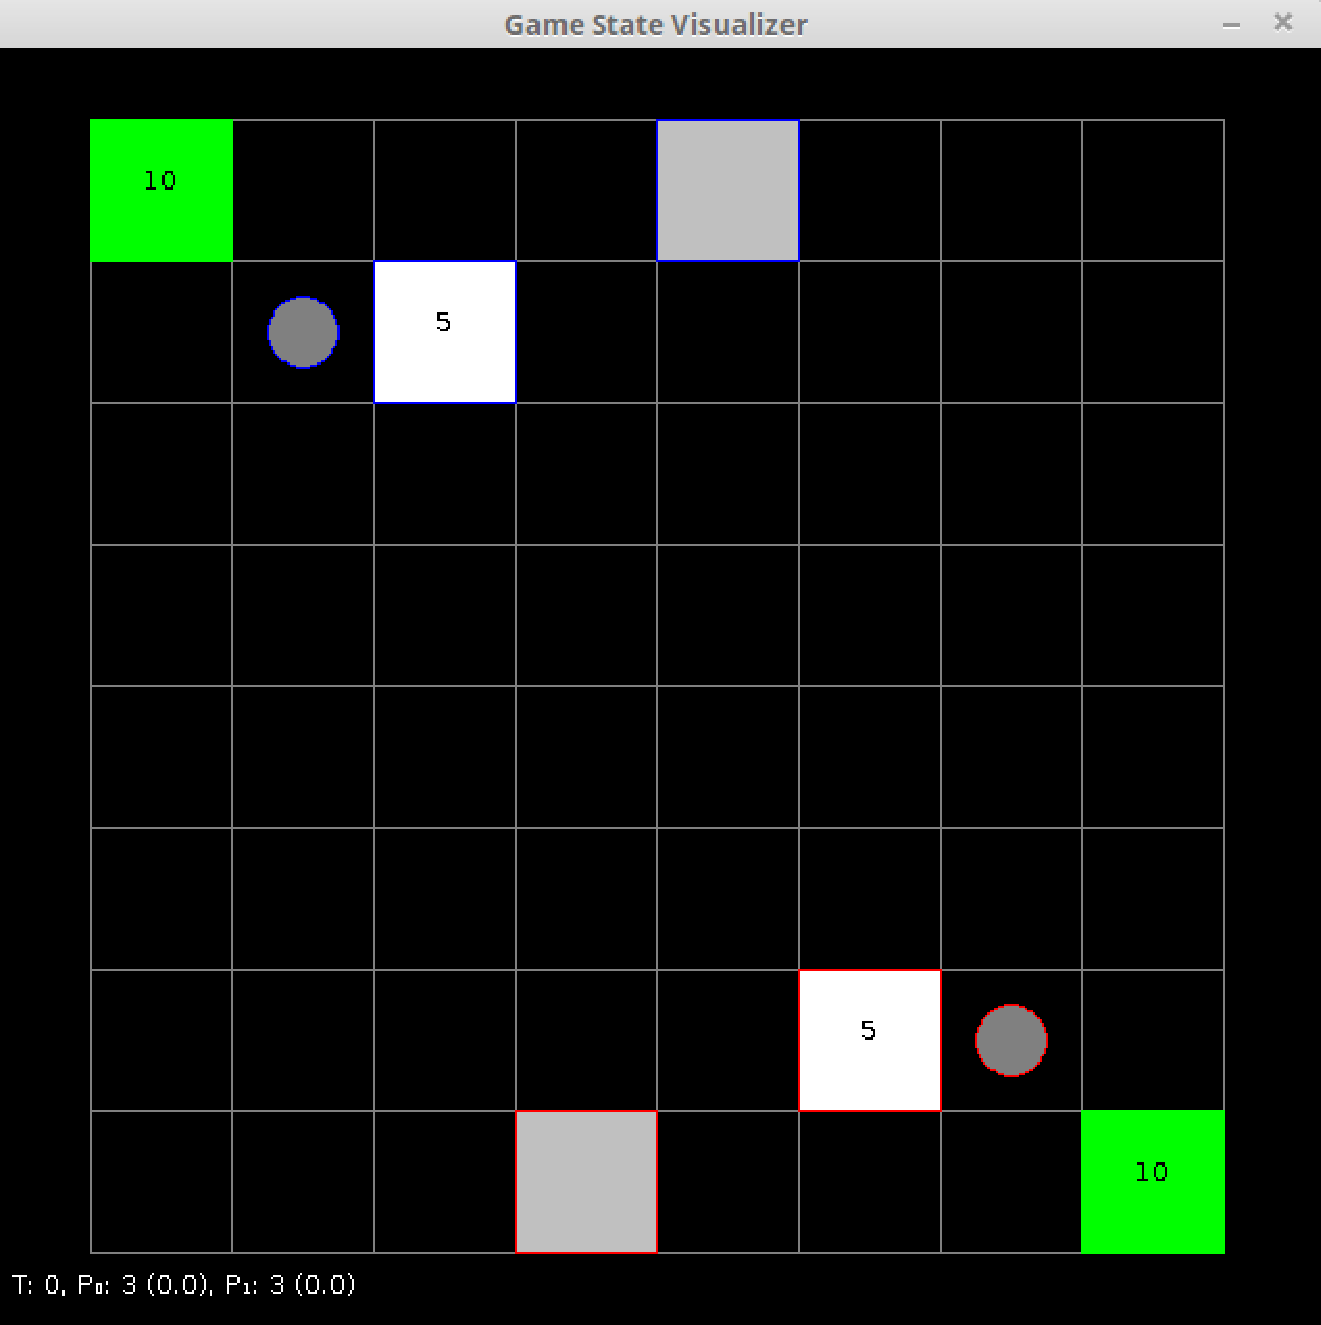
\includegraphics[width=.5\textwidth]{fig/map8x8quartel.pdf}
	\caption{Configuração inicial do mapa 2.}
	\label{fig:mapa8x8quartel}
\end{figure}

A Tabela~\ref{tab:mapa2} ilustra os resultados obtidos neste mapa.
Por conta do mapa ser pequeno em relação ao anterior, não há grande diferença entre os domínios.
O jogo acaba rápido, pois as técnicas criam unidades e logo encontram as unidades adversárias.
Mais uma vez o lado vermelho tem larga vantagem sobre o lado azul. 
Isso acontece pelo fato de que, no lado vermelho, as técnicas do MicroRTS atacam rapidamente, o que não acontece quando as técnicas estão do lado azul, pois após as unidades serem criadas, elas ficam muito tempo paradas antes de atacar.
A técnica do Minimax por exemplo, no lado azul ela cria unidades de ataque mas não envia para atacar, no lado vermelho as tropas são imediatamente postas ao ataque.

\begin{table}[ht]
	\centering
	\caption{Porcentagem de vitórias no mapa 2.}
	\label{tab:mapa2}
	\begin{tabular}{|c|cc|cc|}
		\hline
		\textbf{}           & \multicolumn{2}{c|}{\textbf{Domínio 1}}  & \multicolumn{2}{c|}{\textbf{Domínio 2}}  \\ \hline
		\textbf{Adversário} & \textbf{Lado Azul} & \textbf{Lado Vermelho} & \textbf{Lado Azul} & \textbf{Lado Vermelho} \\ \hline
		RandomIA            & 100\%              & 100\%                  & 100\%              & 100\%                  \\ \hline
		RandomBiasedIA      & 40\%               & 80\%                   & 80\%               & 100\%                  \\ \hline
		RangedRush          & 0\%                & 100\%                  & 0\%                & 100\%                  \\ \hline
		HeavyRush           & 0\%                & 100\%                  & 0\%                & 100\%                  \\ \hline
		LightRush           & 0\%                & 100\%                  & 0\%                & 100\%                  \\ \hline
		WorkerRush          & 0\%                & 0\%                    & 0\%                & 0\%                    \\ \hline
		MonteCarlo          & 0\%                & 0\%                    & 0\%                & 0\%                    \\ \hline
		Minimax             & 0\%                & 100\%                  & 0\%                & 100\%                  \\ \hline
		Portfolio           & 0\%                & 60\%                  & 0\%                & 80\%                  \\ \hline
	\end{tabular}
\end{table}


\section{Mapa 3}

Neste mapa, cada jogador inicia com uma base, um \textit{worker}, e um recurso perto de sua base.
O mapa é composto por 8x8 posições.
Além dos componentes dos jogadores, há posições obstáculos no centro do mapa.
Os obstáculos não são posições validas para os jogadores.
A Figura~\ref{fig:mapa8x8obsta} ilustra a tela do jogo com a configuração inicial do mapa.

\begin{figure}[ht]
	\centering
	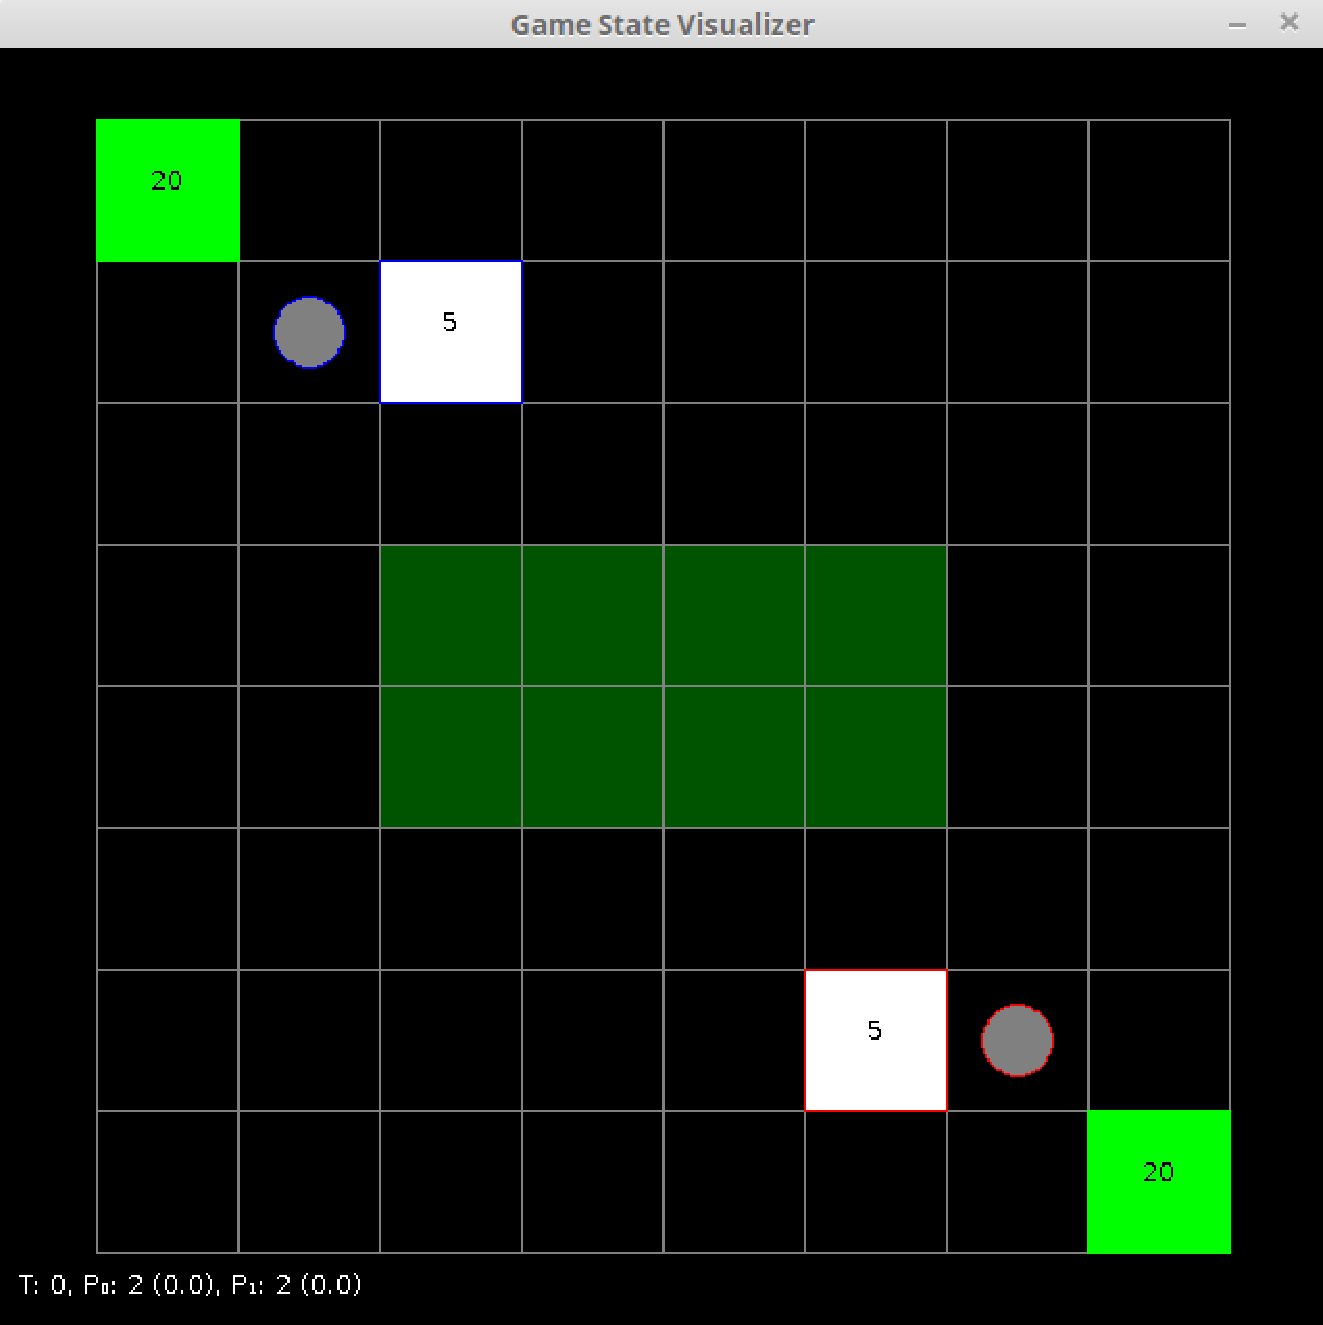
\includegraphics[width=.5\textwidth]{fig/map8x8obsta.pdf}
	\caption{Configuração inicial do mapa 3.}
	\label{fig:mapa8x8obsta}
\end{figure}

A Tabela~\ref{tab:mapa3} ilustra os resultados obtidos neste mapa.
Os resultados mostram, outra vez, a vantagem do lado vermelho no jogo.
Do mesmo modo que no mapa 1, a construção do quartel é mais favorável do lado vermelho.
A colocação de obstáculos no mapa não alterou a maneira com que as técnicas se comportam.

\begin{table}[ht]
	\centering
	\caption{Porcentagem de vitórias no mapa 3.}
	\label{tab:mapa3}
	\begin{tabular}{|c|cc|cc|}
		\hline
		\textbf{}           & \multicolumn{2}{c|}{\textbf{Domínio 1}}  & \multicolumn{2}{c|}{\textbf{Domínio 2}}  \\ \hline
		\textbf{Adversário} & \textbf{Lado Azul} & \textbf{Lado Vermelho} & \textbf{Lado Azul} & \textbf{Lado Vermelho} \\ \hline
		RandomIA            & 100\%              & 100\%                  & 100\%              & 100\%                  \\ \hline
		RandomBiasedIA      & 100\%              & 80\%                   & 100\%              & 80\%                   \\ \hline
		RangedRush          & 0\%                & 100\%                  & 0\%                & 100\%                  \\ \hline
		HeavyRush           & 0\%                & 100\%                  & 0\%                & 100\%                  \\ \hline
		LightRush           & 0\%                & 100\%                  & 0\%                & 100\%                  \\ \hline
		WorkerRush          & 0\%                & 0\%                    & 0\%                & 0\%                    \\ \hline
		MonteCarlo          & 0\%                & 0\%                    & 0\%                & 0\%                    \\ \hline
		Minimax             & 0\%                & 80\%                  & 80\%              & 80\%                   \\ \hline
		Portfolio           & 0\%                & 0\%                    & 0\%                & 0\%                    \\ \hline
	\end{tabular}
\end{table}


\section{Tamanho de cada IA}

Algumas técnicas podem precisar de muito esforço de programação para serem implementadas, já outras podem ser feitas de maneira mais rápida e ter a mesma eficiência.
Uma maneira de comparar as técnicas é através do tamanho do código.
Assim é possível ver o esforço empregado na criação das técnicas.
Pois quanto maior o tamanho, maior o número de linhas de código necessários para a implementação da técnica.
A Tabela~\ref{tab:tamanho} ilustra o tamanho de cada técnica após aplicado um algoritmo de compressão de dados.

\begin{table}[ht]
	\centering
	\caption{Tamanho do código de cada técnica.}
	\label{tab:tamanho}
	\begin{tabular}{|c|c|}
		\hline
		\textbf{Adversário}     & \textbf{Tamanho} \\ \hline
		Domínio HTN 1           & 19,9 kB          \\ \hline
		Domínio HTN 2           & 20,1 kB          \\ \hline
		RandomIA                & 4,0 kB           \\ \hline
		RandomBiasedIA          & 4,6 kB           \\ \hline
		RangedRush              & 13,7 kB          \\ \hline
		HeavyRush               & 14,0 kB          \\ \hline
		LightRush               & 14,0 kB          \\ \hline
		WorkerRush              & 13,6 kB          \\ \hline
		MonteCarlo              & 18,1 kB          \\ \hline
		Minimax                 & 12,9 kB          \\ \hline
		Portfolio               & 14,4 kB          \\ \hline
	\end{tabular}
\end{table}

A implementação do algoritmo de AHTN é a técnica com maior tamanho.
Isso vem do fato de que é preciso integrar com o algoritmo as classes do JSHOP2 e a camada de abstração do MicroRTS.
Fazendo com que o tamanho do código cresça.

A técnica com maior tamanho do MicroRTS é a MonteCarlo.
Contra o algoritmo de AHTN, essa técnica venceu sempre nos mapas 2 e 3, e perdeu no mapa 1 para o domínio 2.
A técnica WorkerRush é a única que não perde em nenhum cenário de jogo.
Ela possui tamanho perto da media dos tamanhos.
As técnicas mais simples, que apenas utilizam movimentos aleatórios, são as técnicas de menor tamanho, e ainda em alguns casos conseguem vencer.

\section{Tempo de geração das ações}

Em jogos RTS, o tempo de geração de uma ação é fundamental.
Técnicas que demoram muito tempo para gerar as ações tendem a ser superadas.
Isso ocorre porque o jogador adversário tem mais tempo para executar suas ações.

A técnica de LightRush foi escolhida como adversário para avaliar o tempo de geração das ações no algoritmo de AHTN.
Essa técnica foi escolhida por ter o mesmo comportamento contra os dois domínios.
O mapa 1 foi o mapa utilizado para este teste.
A Figura~\ref{fig:tempo} ilustra o gráfico com os tempos obtidos para os domínios.

\begin{figure}[ht]
	\centering
	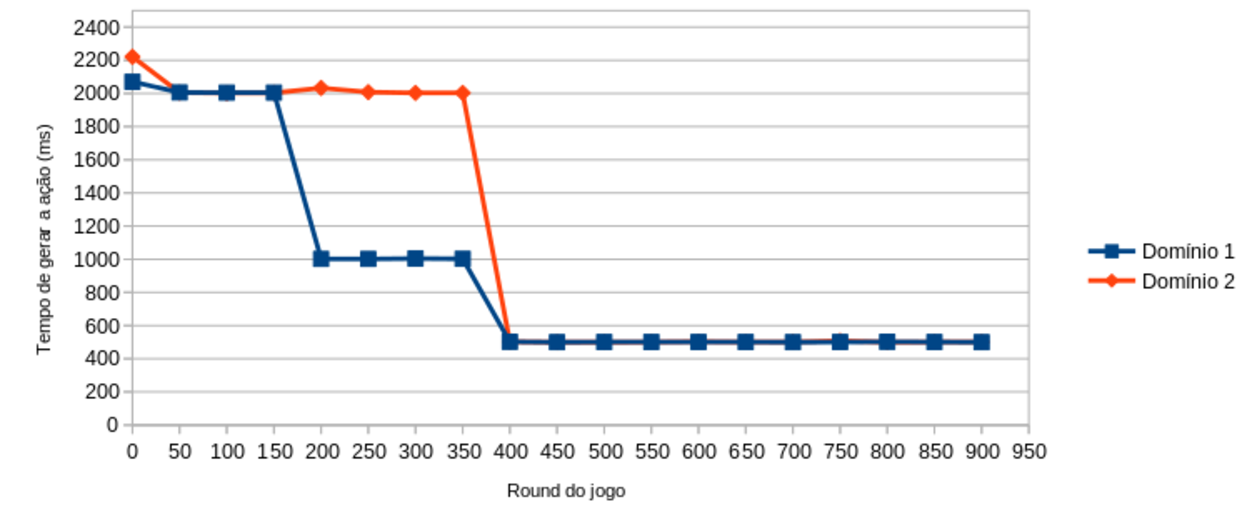
\includegraphics[width=.9\textwidth]{fig/graph.pdf}
	\caption{Tempo de geração das ações para os dois domínios.}
	\label{fig:tempo}
\end{figure}

O gráfico mostra que no inicio do jogo o tempo para gerar uma ação é elevado.
No inicio do jogo, o jogador tem apenas uma base e um \textit{worker}.
Para conseguir vencer o adversário é preciso construir um quartel, e treinar unidades de ataque.
Ao passar das jogadas, o tempo para gerar as jogadas diminui.
Isso ocorre porque há menos ações que podem ser realizadas no jogo, o que implica em menos níveis na árvore de busca que o algoritmo tem que percorrer.
No final do jogo, o jogador já tem tropas de ataque e apenas manda elas atacar.

No domínio 1 o tempo de gerar a unidade de ataque é menor do que no domínio 2.
Isso acontece, pelo fato de que no domínio 1, apenas uma unidade é criada, e com isso os planos gerados são diferentes, já no domínio 2 mais de uma unidade é criada.
O tempo de geração ao final do jogo é semelhante, pois as duas abordagens são parecidas, e se diferem apenas na maneira como as unidades são criadas.

As técnicas do MicroRTS conseguem gerar as ações em poucos milissegundos.
Já o algoritmo de AHTN implementado leva no minimo meio segundo para determinar qual ação deve ser realizada.
Isso ocorre por causa de que a cada troca de perspectiva, o algoritmo tem que gerar os planos novamente.
Pois a cada novo nível na árvore de busca algum componente do ambiente mudou.



%!TEX root = volumeFinal.tex 

\chapter{\label{concl}Conclusões}

%----------------------------------------------------------------
% Após \appendix, se iniciam os capítulos de Apêndice, com
% numeração alfabética.
%----------------------------------------------------------------
\appendix
%!TEX root = volumeFinal.tex 

\chapter{\label{ap:estra1}Domínio HTN da estratégia 1}

\section{Domínio}

\lstset{style=codeStyle}
\begin{lstlisting}[language=lisp]
(defdomain ahtn-estrategia1
	(
		(:operator (!build-base ?worker ?recursoBase)
			((worker ?worker) (have ?recursoBase))
			((have ?recursoBase))
			((base ?base))
		)

		(:operator (!train-worker ?base ?recursoworker)
			((base ?base) (have ?recursoworker))
			((have ?recursoworker))
			((worker ?worker))
		)

		(:operator (!build-barrack ?worker ?recursoQuartel)
			((worker ?worker) (have ?recursoQuartel))
			((have ?recursoQuartel))
			((quartel ?quartel))
		)

		(:operator (!train-ranged ?quartel ?recursoRanged)
			((quartel ?quartel) (have ?recursoRanged))
			((have ?recursoRanged))
			((ranged ?ranged))
		)

		(:operator (!get-resource ?worker ?base ?recurso)
			((worker ?worker) (base ?base))
			()
			((have ?recurso))
		)

		(:operator (!attack-ranged ?ranged)
			((ranged ?ranged))
			()
			()
		)

		(:method (construir-base ?base)
			((not (base ?base)) (recurso ?base ?recursoBase) (have ?recursoBase) (worker ?worker))
			((!build-base ?worker ?recursoBase))
		)

		(:method (treinar-worker ?worker)
			((not (worker ?worker)) (recurso ?worker ?recursoWorker) (have ?recursoWorker) (base ?base))
			((!train-worker ?base ?recursoWorker))
		)

		(:method (construir-quartel ?quartel)
			((not (quartel ?quartel)) (recurso ?quartel ?recursoQuartel) (have ?recursoQuartel) (worker ?worker)) 
			((!build-barrack ?worker ?recursoQuartel))
			
			((not (quartel ?quartel)) (recurso ?quartel ?recursoQuartel) (not (have ?recursoQuartel)) (worker ?worker) (base ?base))
			((!get-resource ?worker ?base ?recursoQuartel) (construir-quartel ?quartel))
			
			((not (quartel ?quartel)) (not (worker ?worker)) (base ?base))
			((treinar-worker ?worker) (construir-quartel ?quartel))
			
			((not (quartel ?quartel)) (not (base ?base)) (worker ?worker))
			((construir-base ?base) (construir-quartel ?quartel))
		)
		
		(:method (treinar-ranged ?ranged)
			((not (quartel ?quartel)))
			((construir-quartel ?quartel) (treinar-ranged ?ranged))
			
			((quartel ?quartel) (recurso ?ranged ?recursoRanged) (not (have ?recursoRanged)) (worker ?worker) (base ?base))
			((!get-resource ?worker ?base ?recursoRanged) (treinar-ranged ?ranged))
			
			((quartel ?quartel) (recurso ?ranged ?recursoRanged))
			((!train-ranged ?quartel ?recursoRanged))
		)
		
		(:method (ataque-ranged ?ranged)		
			((not (ranged ?ranged)))
			((treinar-ranged ?ranged) (ataque-ranged ?ranged))
			
			((ranged ?ranged))
			((!attack-ranged ?ranged))
		)        
	)
)

\end{lstlisting}

%!TEX root = volumeFinal.tex 

\chapter{\label{apendiceB}Domínio HTN da estratégia 2}

\section{Domínio}


\lstset{style=codeStyle}
\begin{lstlisting}[language=lisp]
(defdomain ahtn-estrategia2
	(
		(:operator (!build-base ?worker ?recursoBase)
			((worker ?worker) (have ?recursoBase))
			((have ?recursoBase))
			((base ?base))
		)
		
		(:operator (!train-worker ?base ?recursoworker)
			((base ?base) (have ?recursoworker))
			((have ?recursoworker))
			((worker ?worker))
		)
		
		(:operator (!build-barrack ?worker ?recursoQuartel)
			((worker ?worker) (have ?recursoQuartel))
			((have ?recursoQuartel))
			((quartel ?quartel))
		)
		
		(:operator (!train-ranged ?quartel ?recursoRanged)
			((quartel ?quartel) (have ?recursoRanged))
			((have ?recursoRanged))
			((ranged ?ranged))
		)
		
		(:operator (!get-resource ?worker ?base ?recurso)
			((worker ?worker) (base ?base))
			()
			((have ?recurso))
		)
		
		(:operator (!attack-ranged ?ranged)
			((ranged ?ranged))
			()
			()
		)
		
		(:operator (!train-attack-ranged ?ranged)
			((ranged ?ranged) (quartel ?quartel) (have ?recursoRanged))
			((have ?recursoRanged))
			((ranged ?ranged))
		)
		
		(:method (construir-base ?base)
			((not (base ?base)) (recurso ?base ?recursoBase) (have ?recursoBase) (worker ?worker))
			((!build-base ?worker ?recursoBase))
		)
		
		(:method (treinar-worker ?worker)
			((not (worker ?worker)) (recurso ?worker ?recursoWorker) (have ?recursoWorker) (base ?base))
			((!train-worker ?base ?recursoWorker))
		)
		
		(:method (construir-quartel ?quartel)
			((not (quartel ?quartel)) (recurso ?quartel ?recursoQuartel) (have ?recursoQuartel) (worker ?worker)) 
			((!build-barrack ?worker ?recursoQuartel))
			
			((not (quartel ?quartel)) (recurso ?quartel ?recursoQuartel) (not (have ?recursoQuartel)) (worker ?worker) (base ?base))
			((!get-resource ?worker ?base ?recursoQuartel) (construir-quartel ?quartel))
			
			((not (quartel ?quartel)) (not (worker ?worker)) (base ?base))
			((treinar-worker ?worker) (construir-quartel ?quartel))
		
			((not (quartel ?quartel)) (not (base ?base)) (worker ?worker))
			((construir-base ?base) (construir-quartel ?quartel))
		)
		
		(:method (treinar-ranged ?ranged)
			((not (quartel ?quartel)))	
			((construir-quartel ?quartel) (treinar-ranged ?ranged))
			
			((quartel ?quartel) (recurso ?ranged ?recursoRanged) (not (have ?recursoRanged)) (worker ?worker) (base ?base))
			((!get-resource ?worker ?base ?recursoRanged) (treinar-ranged ?ranged))
			
			((quartel ?quartel) (recurso ?ranged ?recursoRanged))
			((!train-ranged ?quartel ?recursoRanged))
		)
		
		(:method (ataque-ranged ?ranged)
			((not (ranged ?ranged)))
			((treinar-ranged ?ranged) (ataque-ranged ?ranged))
			
			((ranged ?ranged) (quartel ?quartel) (recurso ?ranged ?recursoRanged) (have ?recursoRanged))
			((!train-attack-ranged ?ranged))
			
			((ranged ?ranged) (recurso ?ranged ?recursoRanged) (not (have ?recursoRanged)))
			((!attack-ranged ?ranged) (treinar-ranged ?ranged))
		)        
	)
)


\end{lstlisting}


%----------------------------------------------------------------
% Aqui vai a bibliografia. Existem 3 estilos de citação: use
% 'tcc-alpha' para citações do tipo [Abc+] ou [XYZ] (em ordem
% alfabética na bibliografia), 'tcc-num' para citações
% numéricas do tipo [1], [20], etc., em ordem de referência e
% 'tcc-alpha-full' para citações estilo 'alpha' mas com nomes completos.
%----------------------------------------------------------------
%\bibliographystyle{tcc-alpha-full}
\bibliographystyle{tcc-num}
\bibliography{referencias}



%----------------------------------------------------------------
% Aqui vão os "capítulos" de anexos. Cada anexo deve
% ser considerado um capítulo.
%----------------------------------------------------------------
%\anexos
%\chapter{Meu primeiro anexo}
%\chapter{My second attachment}

% E aqui (para a felicidade de todos) termina o documento.
\end{document}
